\documentclass{article}
\usepackage{amsmath}
\usepackage{amsfonts}
\usepackage{graphicx}
\usepackage{caption}
\usepackage{wrapfig}
\usepackage[utf8]{inputenc}
\usepackage{parskip}
\usepackage{listings}
\usepackage{color}
\usepackage{algorithm}
\usepackage{algpseudocode}

\definecolor{dkgreen}{rgb}{0,0.6,0}
\definecolor{gray}{rgb}{0.5,0.5,0.5}
\definecolor{mauve}{rgb}{0.58,0,0.82}
\definecolor{orange}{rgb}{0.82,0.6,0.4}
\definecolor{black}{rgb}{0,0,0}

\lstset{frame=tb,
  language=Python,
  aboveskip=3mm,
  belowskip=3mm,
  showstringspaces=false,
  columns=flexible,
  basicstyle={\small\ttfamily},
  numbers=none,
  numberstyle=\tiny\color{gray},
  keywordstyle=\color{blue},
  commentstyle=\color{dkgreen},
  stringstyle=\color{mauve},
  identifierstyle=\color{black},
  % numberstyle=\color{blue},
  stringstyle=\color{mauve},
  breaklines=true,
  breakatwhitespace=true,
  tabsize=3,
  escapeinside={(*@}{@*)}
}
\graphicspath{{./Media/Images}}
\setcounter{secnumdepth}{2}

\author{Jack Morgan}
\title{Visualisation of the Riemann Hypothesis}

\begin{document}
\begin{titlepage}
    \begin{center}
    \vspace*{1cm}

    \Huge
    \textbf{An Investigation and Visualisation of the Riemann Hypothesis}

    \vspace{0.5cm}
    \LARGE
    \vspace{1.5cm}

    \textbf{Jack Morgan}

    \vfill

    A-Level Computer Science Coursework\\

    \vspace{2cm}

    \Large
    Dr Challoner's Grammar School\\
    Centre Number: 52205\\
    Candidate Number: 7469\\
    January 2022\\

    \vspace{1cm}

    \end{center}
\end{titlepage}


\section{Analysis}

\subsection{Introduction}

\subsubsection{Project Proposal}

Throughout this coursework, I will be examining the Riemann Hypothesis; to be able to visualise this important conjecture and make its complex mathematical structures accessible for anyone who is interested in mathematics. This project will be heavily based on how to compute and plot recursive mathematical functions on the complex plane and test whether the Riemann hypothesis is a true statement, as well as how the hypothesis affects mathematics today.

\subsubsection{Abstract}

During this coursework, I aim to be able to make the Riemann Hypothesis a more accessible mathematical concept to be able to help people to understand it and hopefully inspire them to research further into related mathematical subjects. I will do this in 3 simple ways:
\begin{enumerate}
\item By detailing what the Riemann hypothesis is and why it is so important,
\item Investigating the major functions that make up the Riemann Hypothesis
\item By Visualising the significant concepts of the Hypothesis, in order to make them more understandable; and to be able to investigate what they are and how they work.
\end{enumerate}

I will be conducting my investigation by programming the key functions of the Hypothesis in Python 3. This will allow me to:
\begin{enumerate}
    \item Compute key mathematical functions
    \item Plot graphs of data
    \item Store data in files and a database
    \item Have a guided user interface
\end{enumerate}

\subsubsection{End Users}

This project is aimed at people who are interested in mathematics. It is a great way to inspire people to delve deeper into maths and number theory; as well as help those with a more advanced understanding of mathematics. Although the mathematics and understanding behind the problem can be complex at times, I am for this project to be able to be used by anyone who will want to use it. This would require it to be simple for people to understand and navigate. I aim to get input from people with a range of mathematical abilities to give me feedback on the project.


\subsection{Research}

\subsubsection{What is the Riemann Hypothesis?}

The Riemann Hypothesis - first proposed by Bernhard Riemann in 1859 - is considered by many to be one the most important unsolved problems in mathematics. To understand why the Riemann hypothesis is so important, it is necessary to understand what the Riemann hypothesis is, and how it is used in many mathematical and scientific fields.
The Riemann hypothesis was proposed by Bernhard Riemann in his paper "On the Number of Primes Less Than a Given Magnitude". This paper deeply explores the prime numbers, and the functions used to estimate and count prime numbers. Throughout this paper, Riemann discussed definitions and proofs of multiple theories that all relate to the prime numbers. But most notably, he had taken a function previously mentioned by Leonhard Euler (a famous mathematician who lived around 100 years prior), and formalised this function into the Riemann Zeta Function.


Riemann took Euler’s function and used a process called analytic continuation to extend the domain of this function to all numbers - be that real, imaginary or complex. Just like every other function, the Riemann Zeta Function contains what are called ‘zeros’ or ‘roots’. This is where a function’s output is equal to zero. These zeros can be described as trivial (where the explanation for why these zeros exist is almost intuitive), or non-trivial (where it can be hard to explain why these zeros occur.) The Riemann Zeta Function has trivial zeros when the input is a negative even integer. I will explore why this is the case later on.

\begin{wrapfigure}{r}{2.1in}
    \centering
    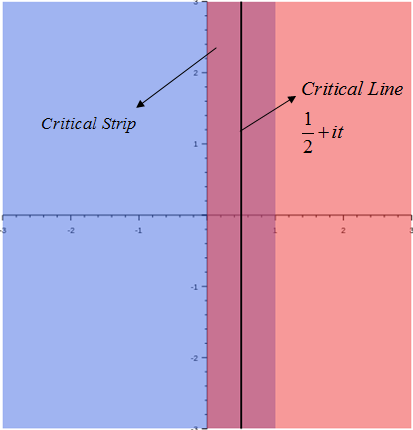
\includegraphics[width=2.0in]{critical-strip}
    \caption{Critical Strip and Line}
\end{wrapfigure}

However, the non-trivial zeros of the zeta function can be found when the real part of the function’s input is between 0 and 1 (called the critical region). This is a fact that has been proven by Riemann in his paper, and he even proved that there are an infinite amount of non-trivial zeros in the critical region. But Riemann went further than this, he hypothesised that the non-trivial zeros do not only occur when the real part of the input is between 0 and 1; but they all occur in the middle of the critical region when the real part of the input is exactly ½. The Riemann Hypothesis states that ‘the real part of every nontrivial zero of the Riemann zeta function is ½’. This is the fundamental part of the Riemann Hypothesis, and although it is widely considered to be true, this conjecture has never actually been proven with conclusive evidence, and that is why these are considered to be non-trivial zeros.


\subsubsection{The Importance of the Riemann Hypothesis}
The Riemann Hypothesis and the  Riemann Zeta Function have many extraordinary uses. From calculating prime numbers to uses in Quantum Physics, and even cryptography with the RSA algorithm. This is due to the fact that the Zeta function is deeply connected to the prime numbers.

One of the main reasons why the Riemann Hypothesis is significant is because there have been many conjectures and theories that assume the Riemann hypothesis to be true. So if the Riemann hypothesis was proven, this would also prove countless other theories.
Some of these theories include :
\begin{itemize}
    \item The weak Goldbach conjecture - stating that all integers greater than 5 are the sum of three primes
    \item Mills’ constants - numbers that allow you to generate prime numbers
    \item The theory that there will always be at least one prime between consecutive cubes
    \item The theory that there is a maximum bound between consecutive prime numbers
\end{itemize}
All of these theories are, in some way, related to the prime numbers. There is an important reason for this which I’ll cover in a later section.

If the Riemann Hypothesis was proven to be true, there would be profound effects in fields such as cryptography. In public-key cryptosystems, like RSA, public keys are created using prime numbers. If someone wanted to try and decode information without knowing what the prime numbers were that created the key, they would have to try and guess what the prime numbers were. What keeps these algorithms secure is the fact that it can take a long time to calculate the prime numbers, especially some of the larger ones. In fact, the largest prime number discovered has over 23 million digits. However, if the Riemann hypothesis were true, then people would be able to calculate the prime numbers much quicker than before. This would make many of the current cryptography algorithms obsolete.

The Riemann Hypothesis does not just influence mathematics and cryptography, it also has great importance in quantum physics. It was discovered in 1996 that the arrangement of the zeta zeros exhibits the same statistical pattern as the spectra of energy levels (that is the possible values of energy of a quantum system) in quantum chaotic systems. Furthermore, it was conjectured in 1999 by Michael Berry and Jonathan Keating, that there will exist a quantum system, where the energy levels will correspond exactly to the non-trivial zeros of the Riemann Zeta Function. If this conjecture is true, it would prove the Riemann Hypothesis.

\subsubsection{Complex Numbers and Key Operations}
Complex numbers play a key part in the Riemann Hypothesis. When Riemann created the Riemann Zeta Function, he allowed the inputs and outputs to be complex numbers, through his ideas of analytic continuation. It is therefore important to know what complex numbers are, and how to do arithmetic with them.

To first understand complex numbers (denoted by the symbol $\mathbb{C}$), it is necessary to be familiar with the idea of imaginary numbers. There is no real number whose square root is a negative number, so mathematicians decided to invent numbers for this. It is denoted by the symbol i, for the imaginary unit.

Where: $$i \equiv \sqrt{-1}$$
And thus: $$i^2 \equiv -1$$
You can multiply the imaginary unit($i$) by any real number to create an imaginary number. For example:
$$3i$$
$$2i$$
Which are both imaginary numbers.
By combining both real numbers and imaginary numbers, you can create complex numbers.
For example:
$$2+3i$$
Where the real part of the number is $2$, and the imaginary part is $3i$.
$$4-7i$$
Where the real part of the number is $4$, and the imaginary part is $-7i$.
We often represent real numbers on a number line, however, this is impossible to do with complex numbers. Instead, one way to understand them is through a two-dimensional graph, or to give it its formal name, the complex plane. On the complex plane, there are two axes, a real axis and an imaginary axis. Any complex number can be plotted on the complex plane. We can think of a complex number as a set of coordinates that tell us where the number lies on the complex plane, with the real part being the x coordinate and the imaginary part being the y coordinate.

So if we wanted to plot the point $2+3i$ on the complex plane, it would look as follows:

\clearpage
\begin{figure}[ht]
    \centering
    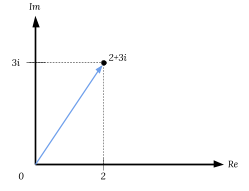
\includegraphics[scale=1]{argand diagram 23i}
    \caption{Argand Diagram of $2+3i$}
\end{figure}

This type of diagram is known as an Argand Diagram. And as you can see, we have plotted the point $2+3i$ at the coordinates $(2, 3)$ on the complex plane.

We can also do arithmetic with complex numbers - be that addition, subtraction, multiplication, division or exponentiation.

The sum of two complex numbers is the sum of both of the real parts of the numbers, plus the sum of the two complex parts of the numbers.
$$(3+2i) + (1+3i)$$
$$= (3+1) + (2i+3i)$$
$$= 4 + 5i$$

Subtraction is also done using a similar method.

$$(3+2i)-(1+3i)$$
$$=(3+2i) + (-1-3i)$$
$$=(3-1)+(2i-3i)$$
$$=2-i$$

To multiply two complex numbers, it is equivalent to expanding out two binomial brackets where:

$$(a+b)(c+d)$$
$$= ac + ad + bc + bd$$

So with two complex numbers this would look like:

$$(3+i)(2+2i)$$
$$= 6 + 6i + 2i + 2i^2$$
$$= 6 + 8i + 2i^2$$

We can then use the identity $i^2 \equiv -1$ to simplify this expression, so that:

$$= 6+8i + 2(-1)$$
$$= 4 + 8i$$

But we can speed up this method by using the rule $(a+bi)(c+di) = (ac-bd)+(ad + bc)i$
For example:
$$(3+i)(2+2i)$$
$$= (3\times2 - 1\times2) + (3\times2 + 1\times2)i$$
$$= 4+8i$$
We can derive this rule, to prove that it works for all complex numbers:
\begin{align*}
    RTP: (a+bi)(c+di) &= (ac-bd)+(ad+bc)i\\
    LHS &=  (a+bi)(c+di)
    \intertext{Distributing Terms:}\\
    &=ac + adi + bci + bdi^2\\
    \intertext{Using $i^2=-1$:}\\
    &=ac + adi + bci -bd\\
    \intertext{Then rearranging:}\\
    &= ac-bd + adi + bci\\
    &= (ac-bd)+(ad+bc)i\\
    &= RHS\\
    &\text{    }Q.E.D
\end{align*}

To divide two complex numbers, we create a fraction and then rationalise the denominator, by using the identity $(a+b)(a-b)  a^2-b^2$ where $a, b \in \mathbb{C}$ (meaning that a and b are both complex numbers)
For example:
\begin{align*}
    (3-i) &\div (2-2i)\\
    &=\frac{3-i}{2-2i}
    \intertext{We can then rationalise the denominator by multiplying the numerator and denominator of the fraction by $(2+2i)$. This does not change the value of the expression but does allow for it to be simplified.}
    &=\frac{3-i}{2-2i} \cdot \frac{2+2i}{2+2i}\\
    &=\frac{(3-i)(2+2i)}{(2-2i)(2+2i)}\\
    \intertext{We can then distribute terms in the numerator and denominator, using the aforementioned multiplication rule:}
    &=\frac{(6+2)+(6-2)i}{4-4i^2}\\
    &=\frac{8+4i}{4-4i^2}\\
    &=\frac{8+4i}{4-(-4)}\\
    &=\frac{8+4i}{8}\\
    &=1-\frac{1}{2}i\\
\end{align*}

There are also some functions that we can use on complex numbers to talk about the real and imaginary parts separately.
The $\Re(z)$ function (also defined as $Re(z)$), outputs the real part of the complex variable $z$. So for example:

\begin{align*}
    \intertext{If we let} z = a+ bi\\
    \intertext{Then} \Re(z) = a
\end{align*}

Similarly, the $\Im(z)$function (also defined as $Im(z)$) outputs the imaginary part of of the complex variable $z$.
For example:

\begin{align*}
    \intertext{If we let} z = a+ bi\\
    \intertext{Then} \Im(z) = b
\end{align*}

Although these functions have limited use in equations and mathematical usage, they prove very handy when needing to discuss complex variables. It is also very useful when computing functions, to be able to split up complex numbers into their real and imaginary parts.

We can also express imaginary numbers using the trigonometric functions, sine and cosine.

Where we have the complex number such that:

\begin{align*}
    z &= a+ bi\\
    \intertext{It can be expressed such that:}
    z &= r \cdot cis(\phi)\\
    \intertext{Where:}
    cis(\phi) &= cos(\phi) + i \cdot sin(\phi)\\
    r =|z| &= \sqrt{a^2+b^2}\\
    \phi =arg(z)&= arctan\left(\frac{b}{a}\right)\\
\end{align*}

This is known as the polar form of the complex number.

We can use this form to easily calculate the value when we raise a complex number to a real power, using De Moivre’s Theorem.
De Moivre’s theorem states that for a complex number in the form


\begin{align*}
    z &= r(cos ( \phi) + i sin ( \phi))\\
    \intertext{If we raise $z$ to the power $n$ then:}
    z^n &= (r(cos(\phi) + i sin(\phi)))^n\\
    &= r^n (cos(n\phi) + i sin(n\phi))
    \intertext{Which is true for}
    &r, \phi, n \in \mathbb{R}, z \in \mathbb{C}
\end{align*}

---- exponentials and factorials -----

\subsubsection{The Riemann Zeta Function}

Previously I have mentioned multiple functions that play a key role in the Riemann Hypothesis, but now I aim to address and examine these functions in detail.

When discussing the Riemann Zeta Function the complex variable $s$ is traditionally used where $s =\sigma  + it$.

The Riemann Zeta Functions is defined as $\zeta(s)$ where:

\begin{align*}
    \zeta(s) &= \sum_{n=1}^{\infty} \frac{1}{n^s}\\
    &= \frac{1}{1^s} + \frac{1}{2^s} + \frac{1}{3^s} + \frac{1}{4^s} + \dots
\end{align*}

This was the equation that Leonhard Euler first introduced and studied, but it was Bernhard Riemann who defined this function for not just all of the real numbers, but all of the complex numbers. Riemann did this through the method of analytic continuation to expand the domain of the function. But by doing it he had to create a new function that would work for all possible input values. He produced what is known as Riemann's Functional Equation:

$$\zeta(s) = 2^s\pi^{s-1}sin\left(\frac{\pi s}{2}\right)\Gamma(1-s)\zeta(1-s) $$
Where $\Gamma(n)$ is the gamma function, such that:

$$\Gamma(n) = \int_{0}^{\infty}n^{s-1}e^{-n} \mathrm{d}n$$

From Riemann's Functional Equation, we can now see why the trivial zeros occur at even negative integers for $s$. This is all due to the sine function. If we let $s = -2n$ for $n \in \mathbb{N}$, (a negative even integer) then the functional equation becomes:

\begin{align*}
    \zeta(-2n) &= 2^{-2n}\pi^{-2n-1}sin\left(\frac{\pi(-2n)}{2}\right)\Gamma(1-(-2n))\zeta(1-(-2n))\\
    \Rightarrow \zeta(-2n) &= -2^{-2n}\pi^{-(2n+1)}sin(n \pi)\Gamma(2n+1)\zeta(2n+1)
\end{align*}
Now we can see that the functional equation includes a factor of $sin(n)$, but due to the nature of the sine function: $sin(n) = 0$ for $n \in  \mathbb{Z}$.  As shown in this diagram of the function $y = sin(x)$:

\begin{figure}[h]
    \centering
    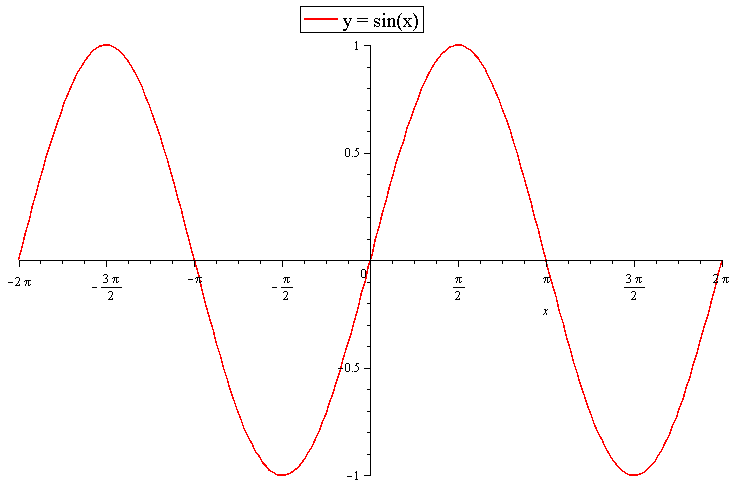
\includegraphics[scale=0.3]{sinx-graph}
    \caption{$y=sin x$}
\end{figure}

And when the sine factor of the functional equation evaluates to zero, this causes the entire function to evaluate to zero, due to the fact that anything multiplied by zero, is zero. This suggests that when s is an even integer, the zeta function evaluates to zero. But then comes the question, why does the zeta function only have zeros at the negative even integers, but not the positive ones? Well, this is because of the gamma function ($\Gamma$).  The factor $\Gamma(1-s)$ in the functional equation has simple poles at positive integers, or in other words, when $s \in \mathbb{N}, \Gamma(1-s)$ is undefined. So for $s \in \mathbb{N}$, the sine function would evaluate to 0, but the gamma function would evaluate to an undefined value. These values cancel each other out, which means that the equation does not necessarily evaluate to $0$ if  $s \in \mathbb{N}$. This is why the trivial zeros are only found at negative even integers.

However, although Riemann’s Functional Equation has significant importance; it is long, complex, and would be hard to compute; mainly due to the fact that it is recursive, with the $\zeta(1-s)$ factor. Luckily, there are other equations that we can use to compute the Zeta function more efficiently.
An example of this is by using the Dirichlet eta function, denoted by $\eta(n)$, such that:


\begin{align*}
    \eta(s) &= \sum_{n=1}^{\infty}\frac{(-1)^{n-1}}{n^s}\\
    \intertext{This function is also known as the alternating zeta function. It has the special property that:}
    \eta(s) &= (1-2^{1-s})\cdot\zeta(s)\\
    \intertext{We can now do arithmetic and rearranging of this function so that we can use it to compute $\zeta(s)$.}
    \intertext{So rearranging for $\zeta(s)$:}
    \zeta(s)&=\frac{1}{1-2^{1-s}}\cdot \eta(s)
\end{align*}


\begin{align*}
    \intertext{Now, if we let $\phi_n = log(n)$, where $log(n)$ is the natural logarithm of $n$, then:}
    n^{it} &= e^{log\left(n^{it}\right)}\\
    &=e^{it\phi_n}\\
    &= cos(t \cdot \phi_n) + i sin(t \cdot \phi_n)
\end{align*}
Then if we express $\zeta(s)$ using $\eta(s)$ in its summation form, and split the variable $s$ into $\sigma+ it$, we derive that:

$$\zeta(\sigma + it) = \frac{2^{it}}{2^{it}-2^{1-\sigma}} \cdot \sum_{n=1}^{\infty} \frac{(-1)^{n-1}}{n^\sigma} \cdot \left[ cos(t\phi_n) -i sin(t\phi_n) \right]$$

Now, this equation is very long and complex, but it seems to be relatively simple to compute.
However, due to the fact that the Dirichlet eta function is only defined for values where the real part of sis greater than one, it means that this form of the zeta function is only defined when $\Re(s) > 0$.

Similarly, we can manipulate the earlier function to find it in another form that will be easy to compute as part of a programaa.
\begin{align*}
    \intertext{If we take the equation from earlier that:}
    \zeta(s)&=\frac{1}{1-2^{1-s}}\cdot \eta(s)\\
    \intertext{And substitute in the eta function where}
    \eta(s) &= \sum_{n=1}^{\infty}\frac{(-1)^{n-1}}{n^s}\\
    \intertext{Then we can say that}
    \zeta(s) &= \frac{1}{1-2^{1-s}}\sum_{n=1}^{\infty}\frac{(-1)^{n-1}}{n^s}
    \intertext{Then, by performing analytic continuation by using Hankel Functions (essentially very complicated mathematics that is beyond the scope of this project), it can be derived that:}
    \zeta(s) = \frac{1}{1-2^{1-s}} \sum_{n=0}^{\infty} & \frac{1}{2^{n+1}} \sum_{k=0}^{n} (-1)^k \binom{n}{k} (k+1)^{-s}
    \intertext{Where $\binom{n}{k}$ is a binomial coefficient where:}
    \binom{n}{k} &= \frac{n!}{k!(n-k)!}
\end{align*}

Just like the previous function we derived, this does look very complicated, however for a computer, it is relatively simple to compute.

$$NEEDS COMPLETING$$
https://mathworld.wolfram.com/RiemannZetaFunction.html
function 21

\clearpage
\subsubsection{The Riemann Hypothesis and Prime Numbers}
The Riemann Hypothesis is deeply connected to the prime numbers. If the Riemann Hypothesis was proven to be true, then the effect this would have on mathematics would be monumental.


Leonhard Euler derived a very nice equation from the Riemann Zeta Function, that involves the prime numbers. This function is known as Euler's Product Formula.

We already know that the zeta function can be defined by:

\begin{align}
    \zeta(s) &= \sum_{n=1}^{\infty}\frac{1}{n^s} \nonumber
    \intertext{Where:}
    \zeta(s) &= \frac{1}{1^s} + \frac{1}{2^s} + \frac{1}{3^s} + \frac{1}{4^s} + \frac{1}{5^s} + \dots \label{1}
    \intertext{Now if we multiply both sides by the second term: $\frac{1}{2^s}$}
    \frac{1}{2^s} \cdot \zeta(s) &= \frac{1}{2^s} + \frac{1}{4^s} + \frac{1}{6^s} + \frac{1}{8^s} + \frac{1}{10^s} + \dots \label{2}
    \intertext{Subtracting equation \ref{2} from equation \ref{1} removes all elements with a factor of 2:}
    \left(1-\frac{1}{2^s}\right) \cdot \zeta(s) &= 1 + \frac{1}{3^s} + \frac{1}{5^s} + \frac{1}{7^s} + \frac{1}{9^s} + \dots \label{3}
    \intertext{Then multiplying again by the second term, $\frac{1}{3^s}$}
    \frac{1}{3^s}\left(1-\frac{1}{2^s}\right) \zeta(s) &= \frac{1}{3^s} + \frac{1}{9^s} + \frac{1}{15^s} + \frac{1}{21^s} + \frac{1}{27^s} + \dots \label{4}
    \intertext{Subtracting equation \ref{4} from equation \ref{3} removes all elements with a factor of 3 as well as those with a factor of 2 from the right-hand side.}
    \left(1-\frac{1}{3^s}\right)\left(1-\frac{1}{2^s}\right) \zeta(s) &= \frac{1}{5^s} + \frac{1}{7^s} + \frac{1}{11^s} + \frac{1}{13^s} + \frac{1}{17^s} + \dots \nonumber
    \intertext{We can see that the right-hand side of the equation is being sieved. If we repeat this process infinitely many times by multiplying by $\frac{1}{p^s}$where $p$ is a prime number, and then subtracting. We end up with:}
    \dots \left(1-\frac{1}{11^s}\right)\left(1-\frac{1}{7^s}\right)&\left(1-\frac{1}{5^s}\right)\left(1-\frac{1}{3^s}\right)\left(1-\frac{1}{2^s}\right) \zeta(s) = 1 \nonumber
    \intertext{Then rearranging for $\zeta(s)$:} \nonumber
\end{align}
$$\zeta(s) = \frac{1}{\left(1-\frac{1}{2^s}\right)\left(1-\frac{1}{3^s}\right)\left(1-\frac{1}{5^s}\right)\left(1-\frac{1}{7^s}\right)\left(1-\frac{1}{11^s}\right) \dots} $$
We can then write this as an infinite product over all primes, $p$:
$$\zeta(s)=\prod_{p, prime} \frac{1}{1-p^{-s}}$$
This function is only defined when $\Re(s) > 0$, due to the fact that negative numbers can not be prime. Furthermore, it would be hard to compute, due to the fact that you would be required to calculate the prime numbers first.

As well as Euler's Product Formula, there are many other functions that involve the prime numbers that are all related to the zeta function.

The prime number theorem was a theorem thought of by Carl Friedrich Gauss near the end of the 18th century. This theorem describes the distribution of the prime numbers. It formalises the intuitive idea that as numbers get larger, the prime numbers are less common, by precisely quantifying the rate at which this occurs. One way this theorem was modelled was through the prime counting function (denoted $\pi(N))$. Where $\pi(N)$ gives the number of primes that are less than or equal to $N$. Given this we can say that as $N \to \infty$ then $\frac{\pi(N)}{log(N)} \to 1$, where $log(N)$ is the natural logarithm of $N$
This, therefore, means that:
$$\pi(N) \sim \frac{N}{log(N)}$$
This means we can approximate the numbers of primes less than or equal to $N$, by calculating $\frac{N}{log(N)}$
For example, if we wanted to approximate the number of primes less than $100$:
Then our approximation would be:
$$\frac{100}{log(100)} = 22$$
But the true value:
$$\pi(100) = 25$$
So there is some error in our approximation.
However, the larger the number $N$, the better our approximation for $\pi(N)$.
For example:

\begin{align*}
    \pi(1,000,000) &= 50,847,534
    \intertext{and}
    \frac{1,000,000}{log(1,000,000)} &= 48,254,942
    \intertext{where proportionally, the error is a lot s      maller}
\end{align*}
However, Peter Dirichlet and Carl Friedrich Gauss came up this a much better approximation for $\pi(N)$. They said that:
$$\pi(N) \sim Li(N)$$
Where $Li(N)$ is the logarithmic integral of $N$ such that:
$$Li(N) = \int_0^N \frac{1}{log(t)} \mathrm{d}t$$
Where $\log(t)$ is the natural logarithm of $t$.
Now if we wanted to use the logarithmic integral function to approximate $\pi(1,000,000)$, we get that:
$$Li(1,000,000) = 50,849,234$$
Which is only $1700$ away from the true value.


As well as the prime counting function, we also have a similar function called the prime power function (denoted by $\Pi(N)$). In the prime counting function, you would get $1$ point per prime number (less than or equal to $N$). But in the prime power function, you get $1$ point per prime $+\frac{1}{2}$ point per prime squared $+ \frac{1}{3}$ point per prime cubed and so on.
As an equation this would be:

\begin{align*}
    \Pi(N) &= \pi(N) + \frac{1}{2}\pi(N^{\frac{1}{2}}) + \frac{1}{3}\pi(N^{\frac{1}{3}}) + \dots \\
           &= \sum_{r=1}^{\lfloor log_2  N\rfloor} \pi(N^{\frac{1}{r}})
\end{align*}

But how is this related to the Riemann Hypothesis? It turns out that the prime number theorem was proved by using the Riemann Zeta Function.

Riemann came up with a function for the Zeta Function where he described it in terms of the non-trivial zeros. He stated:

$$\zeta(s) = \left(\frac{\pi^{\frac{s}{2}}}{2\left(s-1\right)\Gamma\left(\frac{s}{2}-1\right)} \right ) \cdot \prod_{\rho}\left(1-\frac{1}{\rho}\right)$$

Where $\rho$ are the non-trivial zeros of the Riemann Zeta Function.

Then through complex analysis and advanced calculus, it was derived that:
$$\Pi(x) - Li(x) = \sum_{\rho}Li(N^\rho) - log(2) + \int_{N}^{\infty} \frac{1}{t(t^2-1)log(t)} \mathrm{d}t$$

Which tells us the difference or ‘error term’ between the prime counting function, and the prime power function. The main and most influential part of this error term is the sum of the logarithmic integrals of $N^\rho$.

Because $\rho$ are the non-trivial zeros, the non-trivial zeros of the Riemann Zeta function are really controlling the size of this error term. If the Riemann Hypothesis were true and all of the non-trivial zeros lie on the critical strip, then this error term will be as small as possible.

Mathematicians were finally able to prove the prime number theorem by using the Riemann zeta function, by showing that the Riemann zeta function has no zeros on the line $\Re(s) = 1$. However, this error term is controlled by the non-trivial zeros of the Riemann zeta function, and it is still unproven whether all of the non-trivial zeros lie on the critical strip. But if the Riemann Hypothesis were true, then this error term is bounded by:

$$|\pi(N) - Li(N)| \leq c \sqrt{N} \cdot log(N)$$

Where $c$ is some constant

This means that there would also be a similar bound between consecutive prime numbers, such that:

$$p_{n+1} - p_{n} \leq c \sqrt{P_{n}} \cdot log(p_{n})$$

There are also many other consequences if the Riemann Hypothesis was proved to be true. For example, the Weak Goldbach Conjecture would also be proven true, stating that ‘All odd integers greater than 5 are the sum of three primes’. Furthermore, if the Riemann Hypothesis was true then there will always be a prime number between consecutive cubes, such that:

$$x^3 < p < (x+1)^3$$

This would mean that you could define a constant $\theta$ such that $\lfloor \theta^{3^n} \rfloor$is prime for all n. This is called a Mills’ Constant.

All of these theorems and conjectures highlight the importance of the Riemann hypothesis, and that if it was to be proven, it would lead to several major breakthroughs, not only in mathematics but quantum physics and computer science. The fact that the non-trivial zeros of the Riemann zeta function have such an importance in countless other fields just shows how influential the Riemann Hypothesis is.

\subsubsection{Visualisations of the Riemann Hypothesis}

There are numerous ways of visualising functions on graphs and plots. Throughout this next section, I will explore the different types of data visualisation techniques, as well as their positives and negatives.


The most common form of visualisation for the Riemann Hypothesis is showing how the output of the Riemann zeta function varies as you move along the critical strip. It plots the values of $\zeta(s)$ for $s = \frac{1}{2} + it$, where $it$ is some imaginary number.


\begin{wrapfigure}{r}{2.2in}
    \centering
    \captionsetup{justification=centering}
    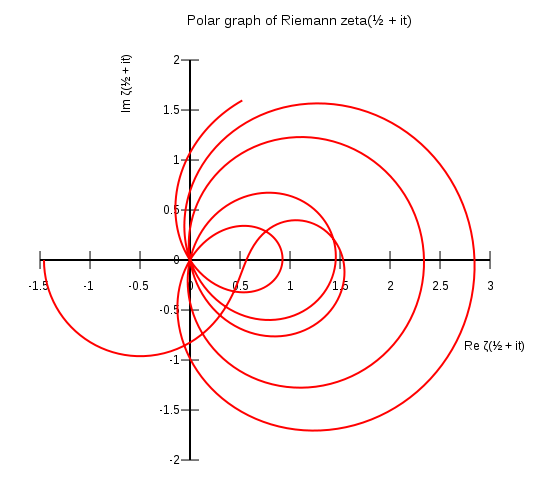
\includegraphics[width=2.0in]{Zeta-Polar-Graph}
    \caption{\\Polar Graph of the Riemann Zeta Function}
\end{wrapfigure}

This graph shows us how the Zeta function varies along the critical strip and allows for us to identify the non-trivial zeros of the function.

Whereas most graphs show the input to the function along a horizontal axis and the output along a vertical axis, we cannot do this with the plot of the Riemann Zeta function because we are required to use both axes to represent complex numbers on the complex plane.

Some positives about this graph are that it is simple and easy to understand. However, it would require an input value for $t$, which is not shown on the graph, for the data to have any practical use.

However, we can expand on this graph and use it to help us to create a dynamic graph. A dynamic graph is one that changes with time. To plot a dynamic graph of the Riemann Zeta function, we could plot values of $\zeta(s)$ along the critical strip so that $\zeta(s) = \frac{1}{2}+ it$. Where $t$ would be our independent variable.

However, we would be changing $t$ over time, where we would need a relationship between the time of the graph and $t$, which could be in the form of an equation.

If for example, we had it so that for every second, the value of $t$ increases by $1$, this would give us a dynamic graph that would plot the points of $\zeta(\frac{1}{2}+it)$ while the user is watching it. The graph would then be changing every second.

If we made it so that for every $0.1$ seconds then t increased by $0.1$, this would give us a much smoother plot and would be much more appealing to look at.

Although the graph at any given point in time would look the same as the previous graph, the fact that this graph is changing for the user to see makes it significantly more visually appealing. Furthermore, by changing the value of $t$ over time, it allows for the user to get a much deeper understanding of how the value of $t$ affects the values of the Riemann Zeta Function.

Another way of representing functions that involve complex numbers is through domain colouring. This technique for visualising complex functions assigns different colours to each point on the complex plane. Not only does domain colouring look very appealing and intriguing it is also very useful to be able to plot functions that require four dimensions.

\clearpage

\begin{wrapfigure}{r}{2.1in}
    \centering
    \captionsetup{justification=centering}
    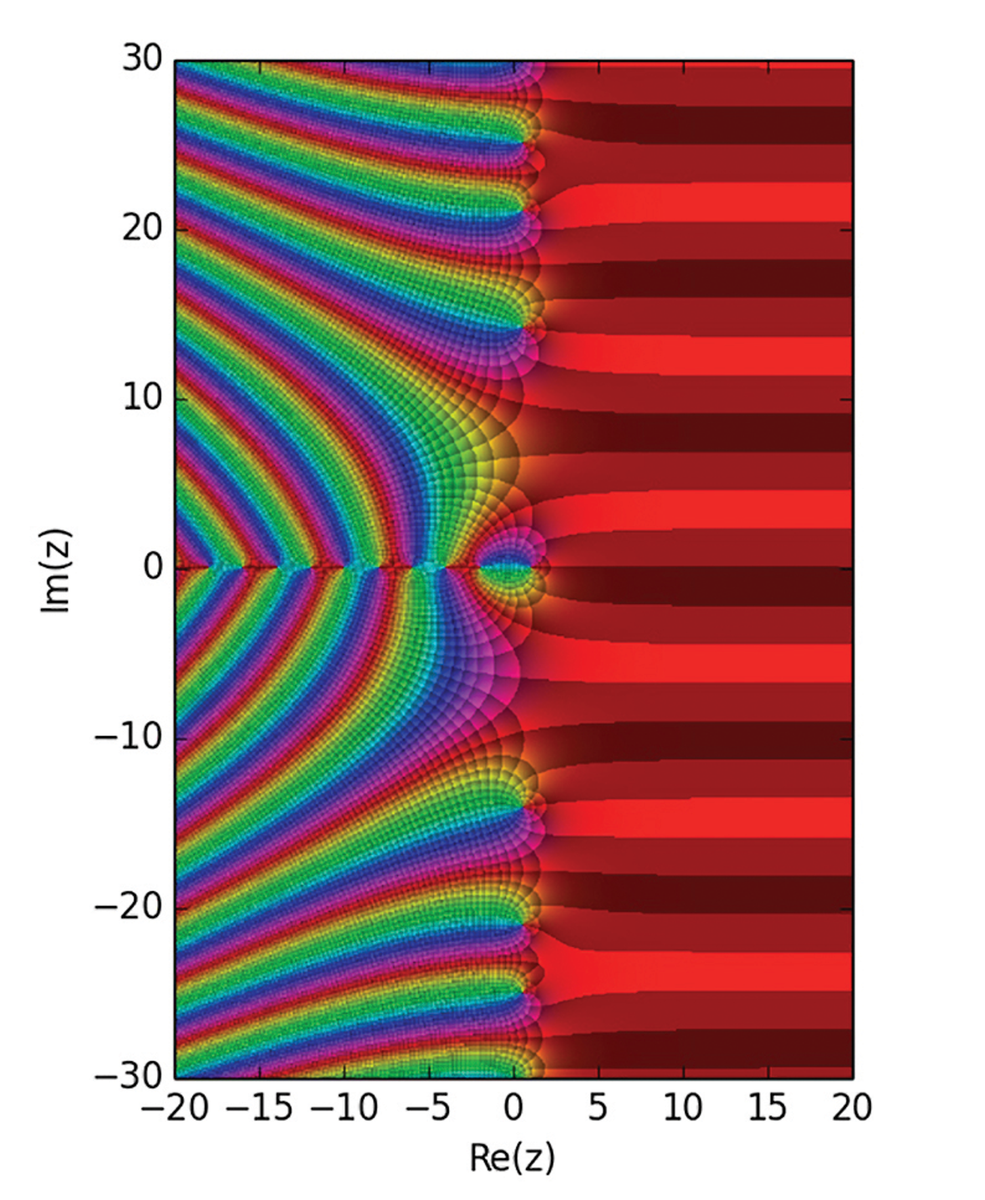
\includegraphics[width=2.0in]{domain-colouring-plot}
    \caption{The Riemann Zeta Function Plotted Using Domain Colouring}
\end{wrapfigure}

To graph a function with real inputs and outputs, two dimensions are required: one for the input and one for the output. But complex numbers are made up of two variables (the real and imaginary parts) and therefore two dimensions.

This means that in order to plot both the input and output of a complex function it requires four dimensions. The simplest way of doing this is by using the method of domain colouring.

In order to represent a function by using domain colouring, it is necessary to determine how the colours of the graph will be chosen.

There are multiple ways of doing this, but one of the most common ways is by taking the output of the function and using this to determine the hue and saturation of the colour.

For example, if we had an argand diagram for the complex number $x+iy$:

\begin{figure}[h]
    \centering
    \captionsetup{justification=centering}
    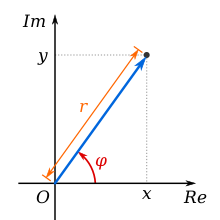
\includegraphics[scale=0.55]{argand-diagram}
    \caption{An argand diagram for the complex number $x+iy$}
\end{figure}

Then we could use the value of $\phi$ to determine the hue of the colour, and $r$ to determine the brightness of the colour.  If we did this for all outputs of a complex function, and then plotted them on a graph, then we would have a domain coloured graph.

Domain coloured graphs have multiple advantages: they look very interesting; they allow complex functions to be plotted using four dimensions; and they are useful to see the general trend of a complex function. However, these graphs are not ideal if you want to read off specific points.

Another method used to illustrate this data is through an interactive graph. An example of this could be where the user selects a complex number on the complex plane. This number is then input into the Riemann Zeta function and an animation is then displayed to show how that number gets translated by the Riemann Zeta Function. The graph would then display another data point that shows the output from the Riemann Zeta Function.

This type of graph is able to show the user how the Riemann Zeta function works and could even give insight into where the zeta zeros could be. Moreover, the interactive feature makes the graph a lot more engaging for the user.


We could also use interactive graphs to show how computers can approximate values for the Riemann Zeta function. Computers are unable to calculate the exact value of the output from the Riemann Zeta function, the reason of which I discuss later on, but it simply comes down to the fact that computers are unable to calculate the infinite series (where an infinite amount of numbers are added together) that are present in the functions. To get around this, you can compute these series to a high number that is not quite infinity, and still get a very accurate approximation.


\begin{wrapfigure}{l}{2.1in}
    \centering
    \captionsetup{justification=centering}
    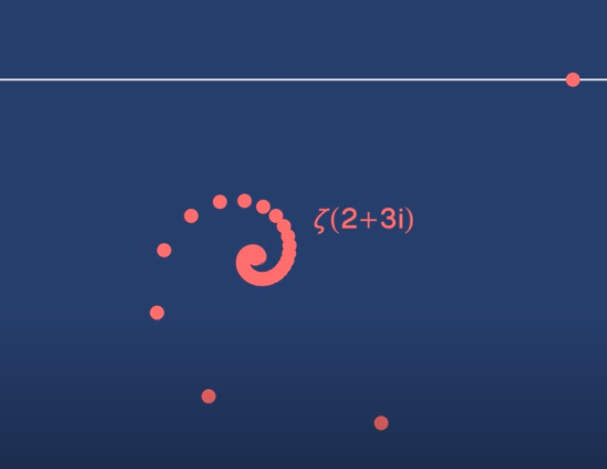
\includegraphics[width=2.0in]{zeta-approximation}
    \caption{The approximation of $\zeta(2+3i)$}
\end{wrapfigure}

As each term in the series gets calculated, the approximation gets closer and closer to the true value. We can use this fact and display it on a graph. If a user selects a point on the complex plane, we can display the approximation for $\zeta(s)$ for $1$ term, $2$ terms ... all the way up until $n$ terms (where $n$ is a high enough number so that the approximation is extremely close to the true value). The resulting graph will show a spiral of data points that converge to one point; that is the output of the zeta function. This graph allows the user to understand how the infinite series works in the zeta function, as well as how computers are able to compute the zeta function.

\subsubsection{Data Storage}

As part of this program, I aim to be able to store the values of the $\zeta(s)$ for specific values of $s$. There are multiple ways to store data sets such as different file types and databases. I will be exploring these data storage methods and finding which method is best suited for my program.

The simplest way of storing data is by storing it in a text (.txt) file. These files store plain text that can be read from and written to. There is limited functionality when it comes to storing data in text files; as you can only read from and write to them. This could be used to store relatively simple and small amounts of data, but to store anything larger and more complex, text files won't be the best choice.

Another way of storing data is by using comma-separated values (CSV) files. These files consist of numerous records and fields, where each line is a record and the fields are separated by delimiters  - often commas.

\begin{wrapfigure}{l}{2.1in}
    \centering
    \captionsetup{justification=centering}
    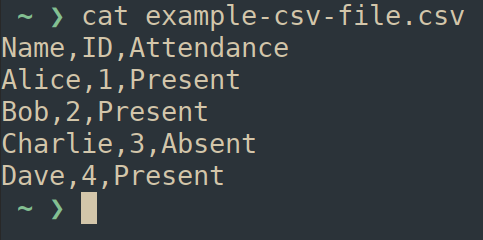
\includegraphics[width=2.0in]{example-csv-file}
    \caption{An example CSV file}
\end{wrapfigure}

This type of storage for data has a lot more functionality than using plain text files. The use of field headers allows entire fields to be read or written to with ease and data can easily be sorted, grouped, and processed. However, some downsides of using the CSV data format are that only basic data can be stored. Complex tables and configurations cannot be used with CSV files. Furthermore, there is no distinction between text and numerical values which can make processing the data difficult.

 Undoubtedly, one of the most efficient ways of storing large data sets is by using databases. More specifically, by using Structured Query Language (SQL).

SQL is a declarative programming language, making it very efficient to use. Databases allow for large amounts of data to be written and read very quickly.

Moreover, processing this data can be very simple with packages such as SQLite that allows SQL databases to be accessed with Python. SQL databases are efficient and can store large amounts of data, making them ideal for a project like this.

\subsubsection{Programming Languages}

There are multiple programming languages that I could - relatively easily -  use for this project, but it is important to choose a language that is suited for the task at hand. Every language has its advantages and disadvantages. Throughout this section I will evaluate various languages and whether or not they would be suitable for this project. I will then give my overall verdict on which language I wish to use.

C++ is a fairly low-level compiled programming language. Its use of classes and memory manipulation allows for an extensive range of functionality. Furthermore, with countless libraries and support, there is almost no limit to what can be done in C++. This is one of the main benefits of this language, alongside the fact that it can run incredibly fast compared to some other interpreted languages, and that it can run on almost any machine. However, the actual coding in C++ is long and tedious. Especially for a project like mine where memory management is not too much of an issue, it seems unnecessary to have to code in C++.

Javascript is also another programming language that could be used for this project. Unlike C++, Javascript is used for more high-level projects, predominantly for web applications.  Making a web app has many advantages, such as high accessibility for multiple users. However, this would require an internet connection to run, and the speed of the program would be significantly reduced compared to that of a compiled application,

Python 3 is a high-level interpreted programming language, with a wide range of libraries and packages to support it. The main advantage of Python is that the code has high readability. This allows for it to be understood by people, even if they are not familiar with the language. Although Python is an interpreted language, there are ways to compile the code into an executable file that can be run on machines that do not have the interpreter installed. As well as this, Python has wide support for user interfaces and the plotting of graphs.

Overall, I think that Python 3 will be the programming language that is most suited for my project. A web application is not what my users are looking for, so javascript would be impractical to use. The high readability and high-level features are what makes Python the optimal programming language for this project, over Javascript and C++.

\subsubsection{Product Research}

Throughout this section, I will be taking a look at other programs that have similar features to mine. I will talk about the advantages and disadvantages of each program and how I can incorporate some of their features into my project.

\begin{wrapfigure}{r}{2in}
    \centering
    \captionsetup{justification=centering}
    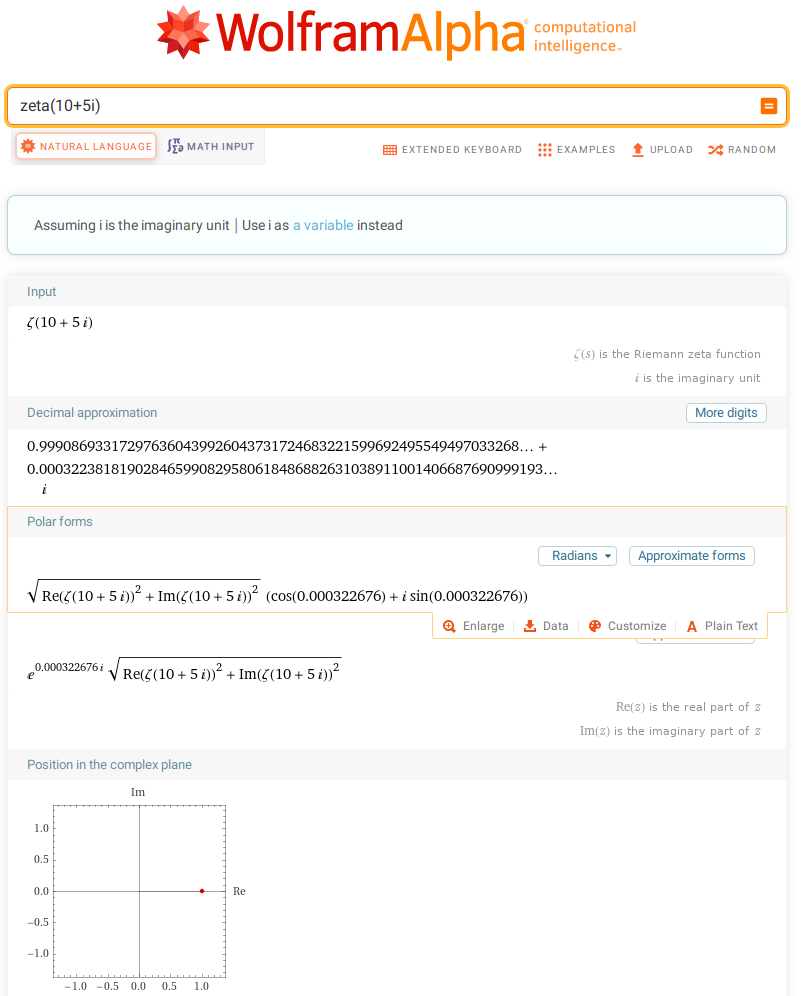
\includegraphics[width=1.9in]{wolfram-alpha}
    \caption{Wolfram Alpha}
\end{wrapfigure}

One of the most major programs I will look at is the web application WolframAlpha. This is a mathematical computation site, where users can input a maths query into a search bar. The answer to the query is then returned, along with information about the solution.

In this example, I input zeta(10+5i). The program then outputs a decimal approximation of the answer to my query, as well as a diagram showing the output on the complex plane. Further down the page, the program lists alternative ways that I could’ve written my input.

This application works very well for calculating specific values of the zeta function, but it does little to show the mathematics of what’s happening to calculate the answer.
\clearpage
Another web application by Wolfram Research is the Riemann Zeta Function Page on Wolfram Mathworld.

\begin{wrapfigure}{l}{2in}
    \centering
    \captionsetup{justification=centering}
    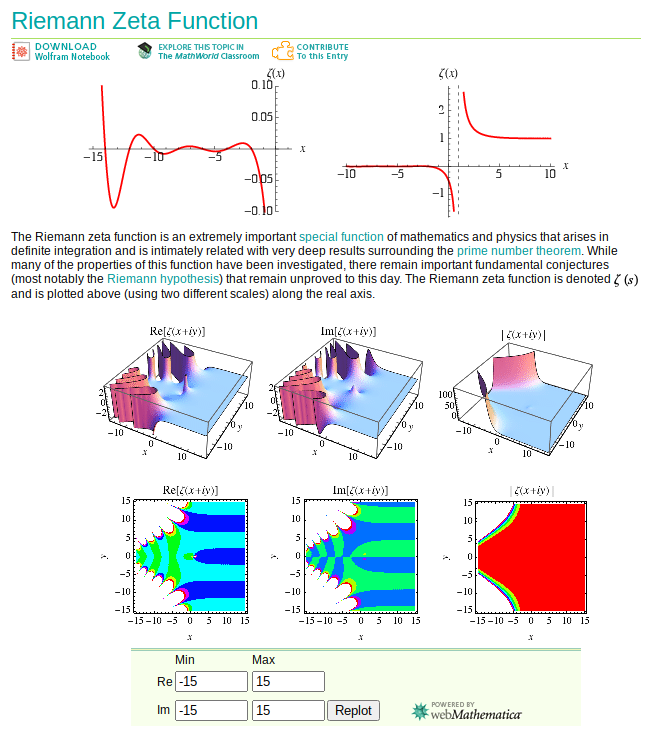
\includegraphics[width=1.9in]{wolfram-mathworld}
    \caption{Wolfram Mathworld}
\end{wrapfigure}

This site explains the Riemann Hypothesis in great detail, giving the user a very thorough understanding of the subject. There are also multiple three-dimensional and domain coloured graphs that plot the Riemann Zeta Function. The user is able to change the scale of the plots to see how the zeta function changes, depending on the input. The web page contains a variety of different graphs and lots of maths along with explanations as to what is going on.

However, the maths on this page is very complex and it would be unlikely that people would understand this page if they didn't have some significant background knowledge into the Riemann Zeta function, or advanced maths in general. The page is also very linear starting from top to bottom. Overall, I like the way that the graphs are presented and explained here, however, the large quantity of maths displayed can seem confusing and unrelated.

\begin{wrapfigure}{l}{2.6in}
    \centering
    \captionsetup{justification=centering}
    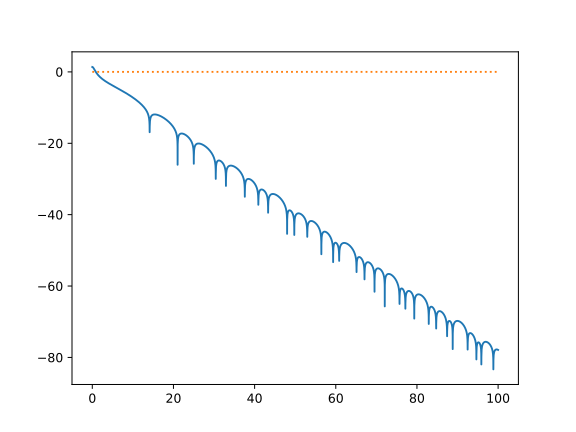
\includegraphics[width=2.5in]{verifying-riemann-hypothesis}
    \caption{Verifying the Riemann Hypothesis by Aaron Meurer}
\end{wrapfigure}

The next program that I will look at is Verifying The Riemann hypothesis by Aaron Meurer.

He creates a program that finds the non-trivial zeros of the zeta function and displays this data on some very simple and understandable graphs. I like this program a lot because it contains a lot of relevant information.

Some positives of this program are that the graphs in it are presented and explained well so that anyone could understand what is going on. The only drawback is that this isn't a very extensive program. Only 2 graphs are calculated and there isn't a user interface.

Overall this program contains some appealing and useful information and graphs but could be more refined.
\clearpage
\subsection{Project Objectives}
My overall aim of this project is to be able to visualise and examine the Riemann Hypothesis, to make the complicated maths more accessible and to test whether the Hypothesis actually is true. I will be doing this by completing the following key objectives.
\begin{enumerate}
    \item The user will be able to use graphs and plots to be able to visualise the Riemann Zeta Function.
    \begin{enumerate}
        \item A visualisation of the convergence of the infinite series.
        \item A graph showing the output value from the Riemann Zeta Function along the critical line
        \item Domain colouring of the Riemann Zeta Function
        \item An interactive graph where the user can choose a point on the complex plane, and the output of the function appears.
    \end{enumerate}
    \item The user will be able to understand the significance of the Riemann Hypothesis and how it is correlated to the prime numbers
    \begin{enumerate}
        \item Plots of the prime counting function, in order to understand the distribution of prime numbers
        \item Graphs showing the Riemann Zeta function as the ‘error term’
    \end{enumerate}
    \item The program will allow the user to calculate values of the zeta function
    \begin{enumerate}
        \item The user will input a number into the calculator
        \item The program will then output the result
        \item A step by step guide of how this answer was calculated will be shown
        \item The user will then have the option to store this information in a database.
    \end{enumerate}
    \item The user will be able to calculate the position of the zeta zeros.
    \begin{enumerate}
        \item The user inputs how many zeta zeros they wish to compute
        \item The program completes the required calculation to find these and outputs the answer to the user
        \item The user will then be able to do multiple things with this data
        \begin{enumerate}
            \item Plot the data to a graph
            \item Store the data in a database
            \item Save the data to a file
        \end{enumerate}
    \end{enumerate}
    \item The program will have a Guided User Interface
    \begin{enumerate}
        \item It will be simple and easily allow for the user to access all parts of the program
    \end{enumerate}
    \item The user will be able to store data that they have collected
    \begin{enumerate}
        \item The program will include a database of multiple results of the zeta function
        \begin{enumerate}
            \item The user will be able to store values of the zeta function
            \item The user will be able to store the non-trivial zeta zeros in the database
            \item The user will be able to retrieve data from the database and display its contents suitably
        \end{enumerate}
        \item The user can store and retrieve data from text files that they can then use in the program.
    \end{enumerate}
\end{enumerate}
\clearpage
\subsection{Third-Party Input}

Throughout the following section, I will be discussing the consultation and guidance that I have received from various third parties. This section will cover the significance of third party input, who my third parties are, how and why I will be conducting my research, a transcript of the actual interviews themselves and my conclusions and takeaways from them.

\subsubsection{The Significance of Third Party Input}
Collecting third party input is vital in creating a successful project. It will allow me to assess the progress that I have made so far in my project, and check that I am heading in the right direction. Having input from various different people allows for people to view the project in different ways, each giving their own advice towards it. Third-party input and feedback is extremely important because it can help me develop and improve my project.

\subsubsection{Who are my Third Parties?}
There are benefits and drawbacks to each person you have as a third party. These depend on their relationship with me, their experience with creating projects like these and their willingness to help; just to name a few factors.

For my third parties, I am using friends who are computer science and further maths students. The benefits of this are that they have good availability, and I can talk to them regularly about the project. Furthermore, they are very supportive and encouraging. Because they are further maths and computer science students, they are also very knowledgeable about the subject area. However, the drawbacks of having friends as third parties are that they are potentially biased towards my project and could be unwilling to criticise it. It could be hard for them to tell me what is wrong, or what could be improved.

\subsubsection{How and Why I will be Conducting My Research}
I will be conducting my third party research by conducting interviews with my third parties. By creating a list of questions, I am able to ask specific questions that are useful to me. I have tailored the questions such that I can use the answers to help improve my project.

The interviews start with me asking questions to the third parties and taking answers from them. At the end of the interview, the third parties have an opportunity to ask me any questions that they have about the project.

\subsubsection{Interview Transcript - Student 1}

\textbf{Question: What will an end-user be able to gain from using this project, how would it be helpful to them?}

Answer: As a maths and further maths student, I want to be able to extend my knowledge of these subjects. This project looks like a good resource that will allow someone to understand the Riemann Hypothesis.

\textbf{Question: What features could be implemented into the project such that the end-users can accomplish what was mentioned in the previous question?}

Answer: It would be very beneficial to the user to have an explanation of the theory behind the Riemann Hypothesis at the beginning of the program. I'd like to do a couple of example steps, so I can try and understand the program before I start using it. You could have an example graph and pause the graphing animation and explain at each point what is happening. As well as this, I would like the program to be interactive so that I can really control what is happening.

\textbf{Question: How accessible would this project be for someone with little or no knowledge of the subject area?}

Answer: Due to the nature of the project, it is not extremely accessible. However, for someone with an interest in mathematics, they may be more willing to research around the topic to gain an understanding

\textbf{Question: What could be done such that people who have less experience with the subject matter are still able to understand the program? How could it still be relevant to them?}

Answer: For people with less experience, you could add some of the background information and story about the Riemann Hypothesis and the investigation. Mention why it's so important, and how it came to be. Not just the maths but the history behind it.

\textbf{Question: Which parts of the project interest you; what would you like to research further?}

Answer: The links to cryptography interest me. The fact it’s such a modern-day feature of life, actually using the function that was theorised so long ago. I am interested in the practical applications of the Riemann Hypothesis and how it actually relates to me.

\textbf{Question: How would someone be able to use this project to extend their knowledge of this subject area?}

Answer: You would be able to use the interactive interface to manipulate and break down the theory of the hypothesis, in order to gain a deeper understanding of it

\textbf{Question: Which features of the project do you like, and why?}

Answer: Visualising is helpful for exploring the project. I like the graphs, the fact it has a visual element is very appealing. It is easier to appreciate the graphs than just looking at mathematical equations.

\textbf{Question: Which features of the project do you think could be improved?}

Answer: The accessibility to the project could be improved; in terms of the mathematics knowledge needed to understand it as well as how the program can be physically accessed and run. For example, as a downloaded piece of software or as a web application.

\textbf{Question: Have you used any similar programs to this? What were they like?}

Answer: A program that seems similar to this that I have used is the practical investigation software Focus eLearning. I used this to carry out practical investigations and consolidate learning. I liked that it was accessible over the internet and that it gave me explanations of the theory, with a visual exploration of the theory it was trying to explain, in the form of the interactive practical experiment. However, I felt that the user interface was difficult to navigate.

\textbf{The question they asked me: How will you refine the access of the project so that everyone can use it?}

My answer: I will include a detailed description and explanation of the Riemann Hypothesis as part of the program to make sure that whatever your mathematical ability, you will still be able to use the program.

\subsubsection{Interview Transcript - Student 2}

\textbf{Question: What will an end-user be able to gain from using this project, how would it be helpful to them?}

Answer: The Riemann Hypothesis itself is used in so many areas such as in cryptography and quantum physics, talking about the practical uses of the hypothesis would be helpful for the user to gain an insight into why the hypothesis is so important.  I am interested in the practical usage of theory in computing and physics. Being able to understand the Riemann Hypothesis visually is also very helpful. Being able to graphically plot the many functions will give a deeper understanding of the project. Furthermore, being able to change the input values to the functions would help so that the user can expand their knowledge of the function

\textbf{Question: What features could be implemented into the project such that the end-users can accomplish what was mentioned in the previous question?}

Answer: It would be very good to make the graphing program interactive. This can be done by changing the function’s input values, but also being able to traverse the plot by scrolling around and zooming in and out by changing the scale. It would also be useful to have multiple graphs displayed on the same set of axes to compare values.

Following along with this interactive idea, I think that you could questions for the user to answer about the hypothesis, to help solidify their understanding of it. It could be beneficial to add sections where the user and write down their observations and any conclusions that they have drawn from the investigation.

To implement this, you could create a login system where a user creates a username and password, so that they would be able to save their progress in the program.

\textbf{Question: How accessible would this project be for someone with little or no knowledge of the subject area?}

Answer: I believe this project will be relatively accessible because it mainly involves just displaying maths functions, where it takes an input and gives an output. It's relatively easy for someone to use it without knowing the details of how it works. That is, to be able to use the program, but maybe not fully understand it. But then to get a deeper understanding of the project, it takes more in-depth knowledge.

\textbf{Question: What could be done such that people who have less experience with the subject matter are still able to understand the program? How could it still be relevant to them?}

Answer: Start off by just exploring and explaining the hypothesis, how it works and how the Riemann zeta function works. If the user wants to understand it further, you can go through the maths of how it works; explaining the Riemann Hypothesis in detail. You could graph the individual mathematical functions in order to break down the problem for the user to understand.  You can use 3D graphs and different ways of representing the data. This could make it easier for the user to understand.

\textbf{Question: Which parts of the project interest you; what would you like to research further?}

Answer: I am very interested in the cryptography application of the Riemann hypothesis. You could showcase as part of this project, a cryptography program that utilises the Riemann hypothesis in a practical way.

\textbf{Question: How would someone be able to use this project to extend their knowledge of this subject area?}

Answer: By utilising the multiple mathematical functions of the Riemann Hypothesis, the user could investigate how changing the input values changes the output. This will help the user learn about the individual functions and their use cases. When combining these functions together, it is important for you to be able to show how changing one piece of data can entirely change the output of a function, especially if the functions are all linked together. You should create the program such that the users could use it to investigate the domains and ranges of the functions.

\textbf{Question: Which features of the project do you like, and why?}

Answer: I like the idea of having an introduction where you explain the practical uses of the Riemann Hypothesis, and where you can give an explanation of how to use the Riemann Hypothesis and Riemann Zeta Function in other programs such as in the RSA cryptosystem. I like how the user would be able to change and manipulate the graphs to their liking and how easy it is to compare values of separate functions. It’s also a good idea to have a  conclusion/summary to help the user fully understand the maths.

\textbf{Question: Which features of the project do you think could be improved?}

Answer: It would be good for the user to be able to draw their own custom graph functions on the same axes as the functions in the program because currently, you would not be able to compare the functions in the program to the user’s own custom functions. A drawback of the project is that the maths could be too specific and intricate for the user to gain a proper understanding of the project. It would require a lot of research to fully understand the project and to be able to make the most of it.

\textbf{Question: Have you used any similar programs to this? What were they like?}

Answer: A program like this that I have used is desmos. Desmos, a graphing software, allows you to plot many graphs on top of each other, you can easily change the axes as well as any input values. What’s bad about desmos is that it doesn’t allow you to plot in 3D, it would be nice to see this in your project. Another program similar to this is Graphing Calculator 3D.
This allows you to do what desmos does, but it plots in 3D. However, its downsides are that It’s not very user friendly and the menus are not easy to navigate, so it can be hard for new users to understand how the software works.

\textbf{Questions asked to me:}

\textbf{Question: What are the necessary system requirements?}

Answer: The necessary system requirements for this program are not very high. The functions are very memory and time efficient so the specifications of the systems that the program is run on should not be an issue.

\textbf{Question: What would help the software be more useful to the user?}

Answer: If that program gave an in-depth explanation of the Riemann Hypothesis, the user can gain a full understanding of what is going on. Furthermore, examples of the practical applications of the Riemann Hypothesis, make the program more relevant to the user and makes this program practical use instead of just being theory.

\textbf{Question: With such complicated functions, how long would it take to compute them?}

Answer: The functions I have written are very memory and time-efficient, it will not take an extensive amount of time to compute the required mathematical functions.

\textbf{Question: To what degree of accuracy will the functions be plotted?}

Answer: The user will have an option where they can increase or decrease the accuracy of the functions. However, this will come with the disadvantage that it will take longer to compute.

\subsubsection{Interview Conclusion}
There are multiple improvement points from these interviews that I have used to help develop the plan for my project.

One of my main improvement points is with the design and layout of the project. The program will have 3 main sections: the introduction, the investigation, and the summary.

The introduction section will let the user be able to read and learn about the Riemann Hypothesis, so they can get an understanding of it, before using the main program. This introduction aims at making the program more accessible to people, even if they have less experience with maths. It will also allow people to explore the Riemann Hypothesis’ links to cryptography and other practical applications so that they can explore it in more detail.

After the introduction will be the actual practical investigation, this is where the user can plot graphs and really investigate the Riemann Hypothesis. They will be able to plot multiple graphs on the same axes in order to be able to compare values. The user will also be able to easily change the input values to many of these graphs so that they can investigate how this changes the outputs.

The final part of the program will be a summary; showcasing the results from the investigation that they have conducted, and detailing some of the key mathematics behind the investigation.

Breaking down the project into these three sections will allow for the User Interface of the program to be simple, such that the user can access all of the relevant parts of the program easily.

Another part of the project spoken about in these interviews was a login system to help save a user's progress through the program. There would be multiple points in the program where the user can answer questions about the hypothesis to check understanding, or for the user to just write down any conclusions that they make about the investigation and the Riemann Hypothesis. Thus, creating a login system would allow a user to save their progress in the program, and any of their answers and data can be stored in a database.
\clearpage
\subsection{Modelling the Problem}
In this section, I will report any modelling of my project that will inform the design stage. I will be covering how to compute certain mathematical functions and also try some prototypes for what the project will look like.

\subsubsection{Prototypes}

Throughout this next section, I will be prototyping some mathematical functions in Python that will allow me to compute the Zeta Function. I will then test each of the functions to make sure that they work as expected.

The majority of functions that I intend to use involve an infinite sum, which is something that we are unable to compute because it would be impossible to add up an infinite amount of numbers. Therefore we must approximate the value of the function by calculating it for a certain number of terms. For example, when calculating the zeta function where:

$$\zeta(s) = \sum_{n=1}^{\infty} n^{-s}$$

We can approximate the value but calculating the sum to such a high number, that the error difference is not significant. If we want to approximate the zeta function, we could compute:

$$\zeta(s) = \sum_{n=1}^{1x10^6} n^{-s}$$

Which would not give us the exact value, but one close enough that we can still use.

First of all, is a function that computes the zeta function by its definition. $\zeta(s) = \sum_{n=1}^{\infty} n^{-s}$. This function is defined for $\Re(s) > 1$ and could look as follows in Python 3:

\begin{lstlisting}
# calculates zeta(s) for any complex number where Re(s) > 1
# where \zeta(s)=\sum _{n=0}^{\infty }\frac{1}{n^s}
def zeta(s: complex) -> complex:
    TERMS = 5 * 10**3 # the number of terms that we wish to compute.
    result = 0
    # computes an approximation for the infinite sum
    for n in range(1, TERMS+1):
        result += 1/(n**s)
    # output the final result
    return result
\end{lstlisting}

First, we define the function \textit{zeta(s)}, where \textit{s} is a complex variable. Then the constant \textit{TERMS} is defined then defined to be a large integer. This number determines how many times we calculate $\frac{1}{n^s}$ and therefore determines how accurate our approximation will be. Then in the for loop, we calculate $n^{-s}$ for \textit{TERMS} many times and sum it to our result. We then return the complex variable res in order to output from the function.

Here we can test the function to show if and when it works as expected, and also how accurate it is to the true value.
\\
\begin{table}[ht]
    \centering
    \begin{tabular}{|c|c|c|c|c|c|c|}
    \hline
    \textbf{No.} & \textbf{Type} & \textbf{Input} & \textbf{Expected Output} & \textbf{Output} & \textbf{Result}\\
    \hline
    \hline
    1 & Invalid & -1 & ValueError & 12502500.0 & Fail\\
    \hline
    \multicolumn{2}{|c|}{Comment} & \multicolumn{4}{|c|}{This output is neither the output we were expecting}\\
    \multicolumn{2}{|c|}{} & \multicolumn{4}{|c|}{nor the correct output of $\zeta(-1)$. I will need to fix}\\
    \multicolumn{2}{|c|}{} & \multicolumn{4}{|c|}{this by validating the input to check that it is}\\
    \multicolumn{2}{|c|}{} & \multicolumn{4}{|c|}{within the defined range of the function}\\
    \hline
    \hline
    2 & Invalid & 0 & ValueError & 5000.0 & Fail\\
    \hline
    \multicolumn{2}{|c|}{Comment} & \multicolumn{4}{|c|}{This is the same situation as test number 1}\\
    \hline
    \hline
    3 & Boundary & 1 & ValueError & 9.095 & Fail\\
    \hline
    \multicolumn{2}{|c|}{Comment} & \multicolumn{4}{|c|}{This is the same situation as the previous tests}\\
    \hline
    \hline
    4 & Valid & 1.5 & 2.61 & 2.584 & Fail\\
    \hline
    \multicolumn{2}{|c|}{Comment} & \multicolumn{4}{|c|}{Although this gives an output that is close to the}\\
    \multicolumn{2}{|c|}{} & \multicolumn{4}{|c|}{expected output, it is not accurate enough. I need}\\
    \multicolumn{2}{|c|}{} & \multicolumn{4}{|c|}{to increase the number of terms in order to get a}\\
    \multicolumn{2}{|c|}{} & \multicolumn{4}{|c|}{more accurate output}\\
    \hline
    \hline
    5 & Valid & $5$ & $1.025$ & $1.025$ & Pass\\
      & & $+10i$ & $-0.015i$ & $-0.015i$  & \\
    \hline
    \multicolumn{2}{|c|}{Comment} & \multicolumn{4}{|c|}{This test gives a value that is extremely close to the}\\
    \multicolumn{2}{|c|}{} & \multicolumn{4}{|c|}{true value. It see,s that out approximation becomes}\\
    \multicolumn{2}{|c|}{} & \multicolumn{4}{|c|}{more accurate as the input value increases.}\\
    \hline
    \end{tabular}
\end{table}
\clearpage
Based on the testing, I have made some adjustments to the function as seen here:

\begin{lstlisting}
# calculates zeta(s) for any complex number where Re(s) > 1
# where \zeta(s)=\sum _{n=0}^{\infty }\frac{1}{n^s}
def zeta(s: complex) -> complex:
    # validate that Re(s) > 1
    if not s.real > 1:
        raise ValueError('Real part of input must be greater than 1')
    TERMS = 1 * 10**6 # the number of terms that we wish to compute.
    result = 0
    # computes an approximation for the infinite sum
    for n in range(1, TERMS+1):
        result += 1/(n**s)
    # output the final result
    return result
\end{lstlisting}

The first change I made was validating the input. Now if the real part of the input is less than $1$, then a \textit{ValueError} is raised. Secondly, I have increased the number of \textit{TERMS} that are computed in order to make the program more accurate. Although this does make the program take more time, the time difference is hardly noticeable.

Now here are the testing results for the improved function.

\begin{table}[ht]
    \centering
    \begin{tabular}{|c|c|c|c|c|c|c|}
    \hline
    \textbf{No.} & \textbf{Type} & \textbf{Input} & \textbf{Expected Output} & \textbf{Output} & \textbf{Result}\\
    \hline
    \hline
    1 & Invalid & -1 & ValueError & ValueError & Pass\\
    \hline
    \multicolumn{2}{|c|}{Comment} & \multicolumn{4}{|c|}{This works as expected; the error is raised}\\
    \hline
    \hline
    2 & Invalid & 0 & ValueError & ValueError & Pass\\
    \hline
    \multicolumn{2}{|c|}{Comment} & \multicolumn{4}{|c|}{This works as expected; the error is raised}\\
    \hline
    \hline
    3 & Boundary & 1 & ValueError & ValueError & Pass\\
    \hline
    \multicolumn{2}{|c|}{Comment} & \multicolumn{4}{|c|}{This works as expected; the error is raised}\\
    \hline
    \hline
    4 & Valid & 1.5 & 2.61 & 2.61 & Pass\\
    \hline
    \multicolumn{2}{|c|}{Comment} & \multicolumn{4}{|c|}{This functions output is very close to the true value}\\
    \hline
    \hline
    5 & Valid & $5$ & $1.025$ & $1.025$ & Pass\\
      & & $+10i$ & $-0.015i$ & $-0.015i$  & \\
    \hline
    \multicolumn{2}{|c|}{Comment} & \multicolumn{4}{|c|}{This functions output is very close to the true value}\\
    \hline
    \end{tabular}
\end{table}

Overall, this function is able to compute values of $\zeta(s)$ where $\Re(s) > 1$. It throws an error at incorrect inputs (which is good) and calculates $\zeta(s)$ relatively accurately. However, this approximation could be made more accurate by increasing the number of \textit{TERMS}, although this could slow the program down significantly. Using this function to calculate $\zeta(s)$ to any useful degree of accuracy would take too much time to compute. Furthermore, this function only allows us to calculate values where $\Re(s) > 1$.

\clearpage
\section{Documented Design}

\subsection{Structure Diagrams}

The program will be made up of 4 main parts; that is the Login System, the Introduction, the Investigation, and the Summary.

The login system will allow users to either sign into an account or create an accoun with a username and password. All user information will be encrypted using hashing algorithms for security reasons, and the data will be stored in a database. The purpose of the login system is to allow the users to save their progress throughout the program. There will be various opportunities throughout the program for the user to write down answers to questions, or to record any observations that they make. This data will be stored specifically to their username such that when they next log in, they can continue from where they left off.

The introduction will be a visual section of the project that will demonstrate to the user how the program will work, as well as give an overview of what the riemann hypothesis is, why it's important, and how it is used in science and technology. The aim of this section is to provide the user with sufficient information and knowledge such that they will be able to effectively be able to use this program. Because quite a lot of mathematical knowledge is required to be able to properly use this program to its full potential, this section will try and provide some basic information of the project area for the user to feel more comfortable using the program.

The investigation will be the main bulk of the program. It will allow the user to plot graphs, find zeta zeros using a variety of methods, and investigate how prime numbers are related to the zeta function. The aim of this section is to get the user to investigate the hypothesis, collecting their own data that they can draw conclusions from.

Finally, the summary will be the last section of the program. Its purpose is to allow the user to reflect on their results, and see what conclusions they are able to draw from them. The summary will be split into 4 sections; a quick recap of the theory from the introduction section; followed by an overview of the user’s results from the investigation. There will then be sections on whether their data proves/ disproves the Riemann hypothesis, how reliable the information from this program will be, and the impact on maths and computer science if the hypothesis is proven to be true.
\clearpage
\subsubsection{Program Overview Structure Diagram}
The following structure diagram for the program gives an overview of the main sections in the project:

\begin{figure}[ht]
    \centering
    \captionsetup{justification=centering}
    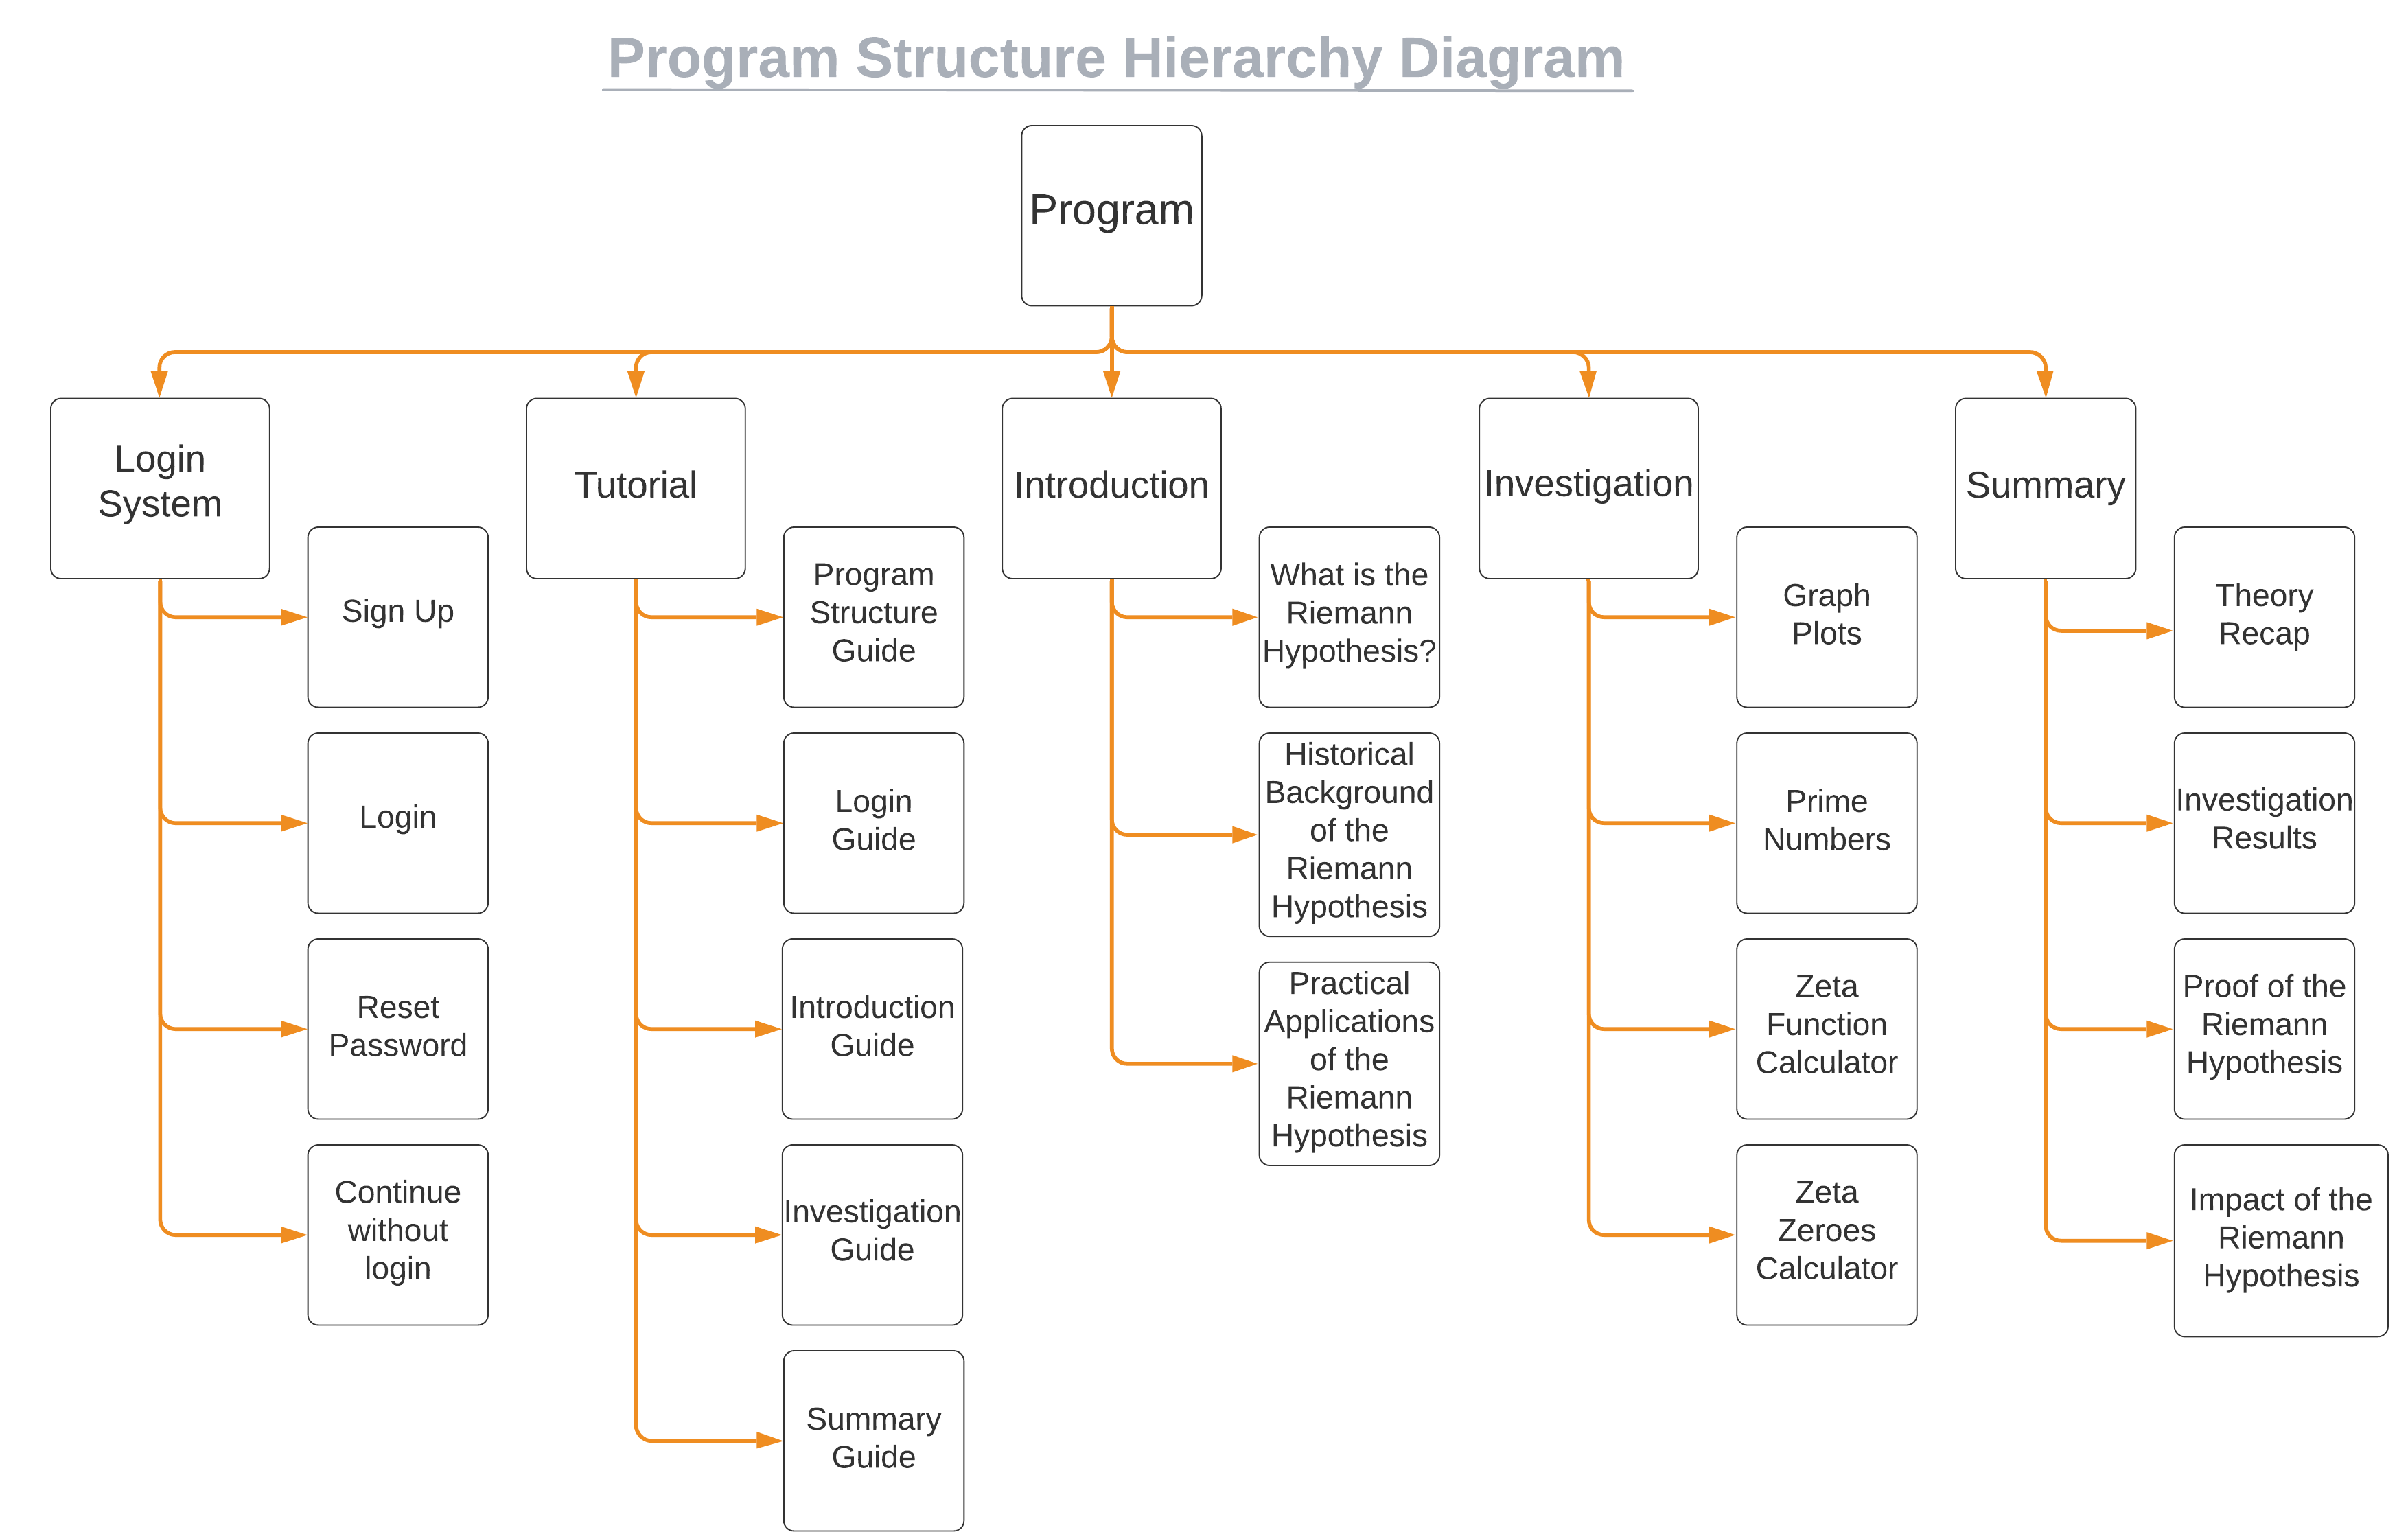
\includegraphics[scale=0.095]{program-structure-hierarchy-diagram}
    \caption{Structure Diagram for the program}
\end{figure}

As we can see from this diagram; the main program is split up into its 5 main sections: the Login System, the Tutorial, the Introduction, Investigation, and the Summary. Each of these main sections is then further broken down into its relevant subsections.

We can then break down each section into its subsections, which will in turn, be broken down into more sections.
\clearpage
\subsubsection{Login System Structure Diagram}

The login system's aim is to be able to allow a user to sign into an account, such that their progress with the program has been kept.

It will not be necessary for a user to login, however, if they do not log in, then their progress will not be saved.

\begin{figure}[h]
    \centering
    \captionsetup{justification=centering}
    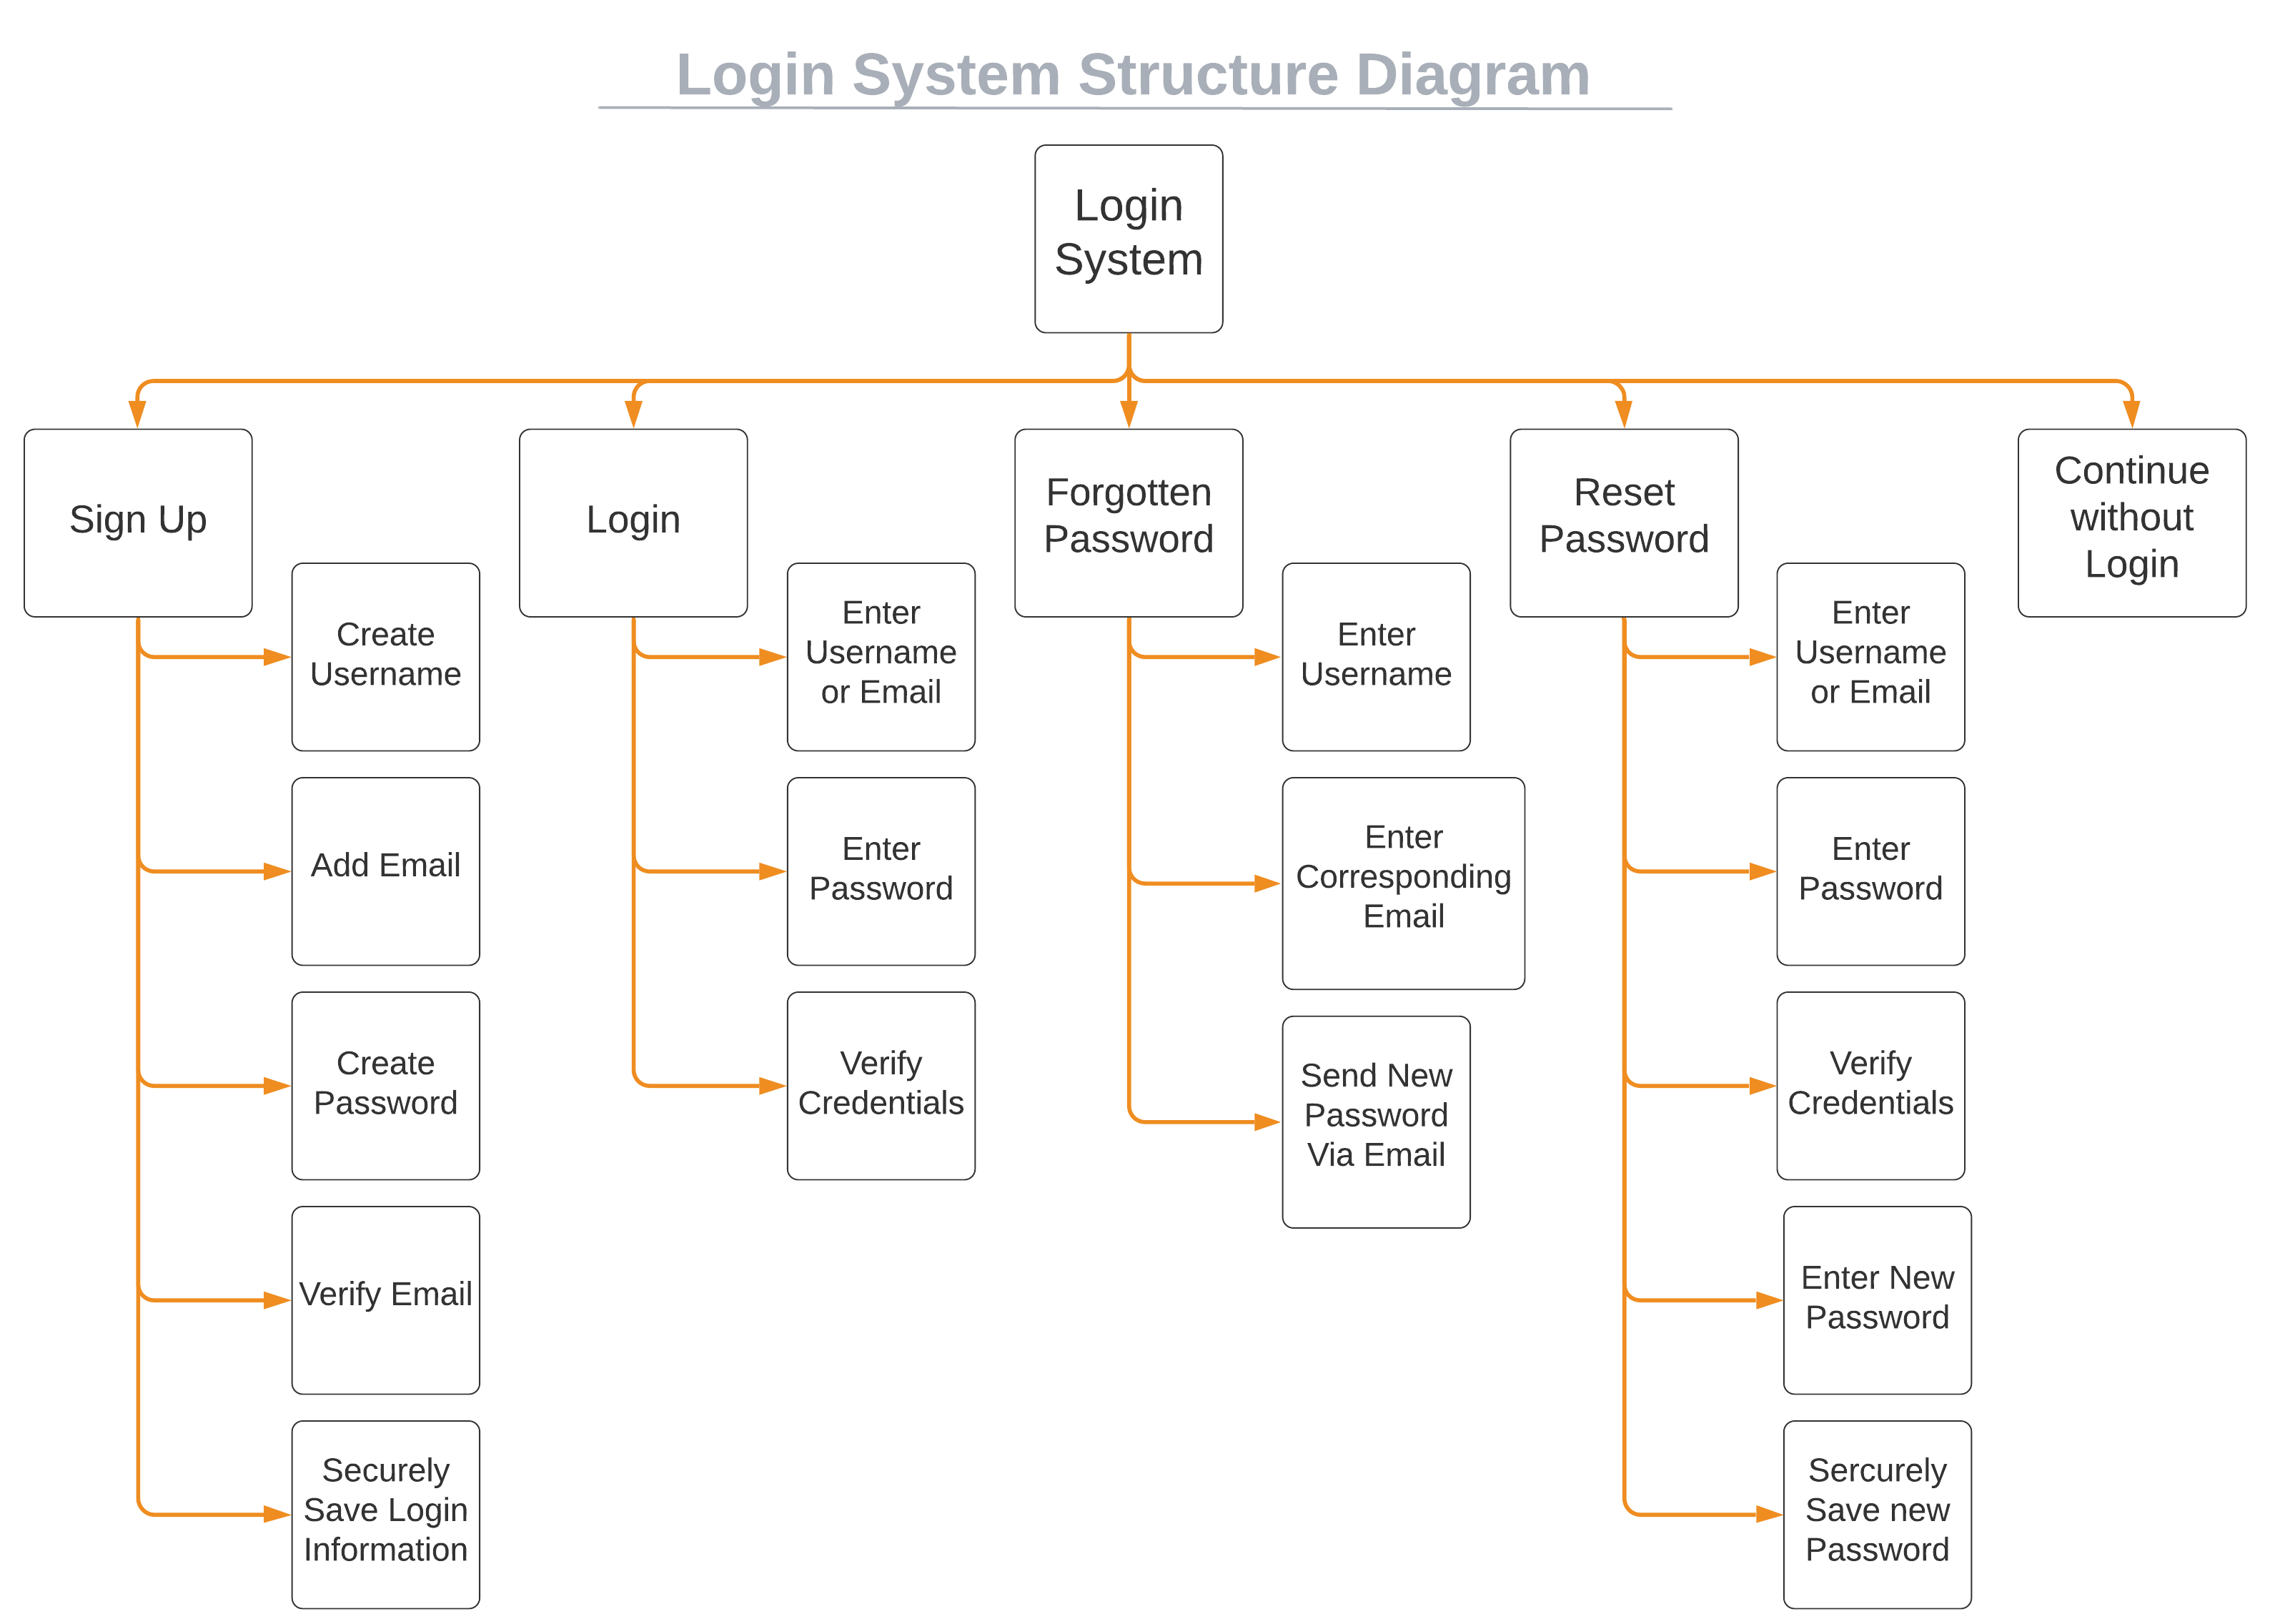
\includegraphics[scale=0.45]{login-system-structure-diagram}
    \caption{Login System Structure Diagram}
\end{figure}

There will be 5 sections to the login system that I create. The first of which allows the user to sign up and create an account. This is for first-time users of the programme, who want to be able to use it to its full functionality. The sign up process involves the user creating a unique username, adding a unique email to the account (used for when the user forgets their password), and creating a strong and complicated password. They will then be sent an email to the address that they entered, with a verification code. Once this code has been entered in the program, the user's login details will be encrypted and stored in a database. They will then advance to the next part of the program: the tutorial.

The login section will allow the user to sign in to an account that has already been created. They will be required to enter either their username or email, and their password. The program will check whether the username or email is valid (if it is in the database), and if the password associated to that account is the same as the one entered by the user. If the user gets the password wrong 3 times, then they will have to wait 1 minute before trying again. This is to stop any attacks to try and guess user's passwords. Once a user has signed in, they will be taken to the tutorial section.

If a user has forgotten their password, then they will be able to reset it in the forgotten password section. The user will be required to enter either their username and email for that account. These credentials will need to be verified, and then if they are correct, a new password will be sent to the user by email.The user will then be sent straight to the Reset Password screen so that they can change the password to one that they will remember.

The reset password section will allow the user to change their password if they don't like the one they currently have, or if they have had to reset their password. They will have to enter their username and password, to confirm their identity. They will then enter a new strong and complicated password, and this will be the new password associated to their account.

The final section is the continue without login section. Without a login, the user will still be able to use all parts of the program, however, their data will not be saved.

\subsubsection{Tutorial Structure Diagram}

The tutorial is one of the key sections of the program. The tutorial will give the user a guide on how to use the program.

\begin{figure}[h]
    \centering
    \captionsetup{justification=centering}
    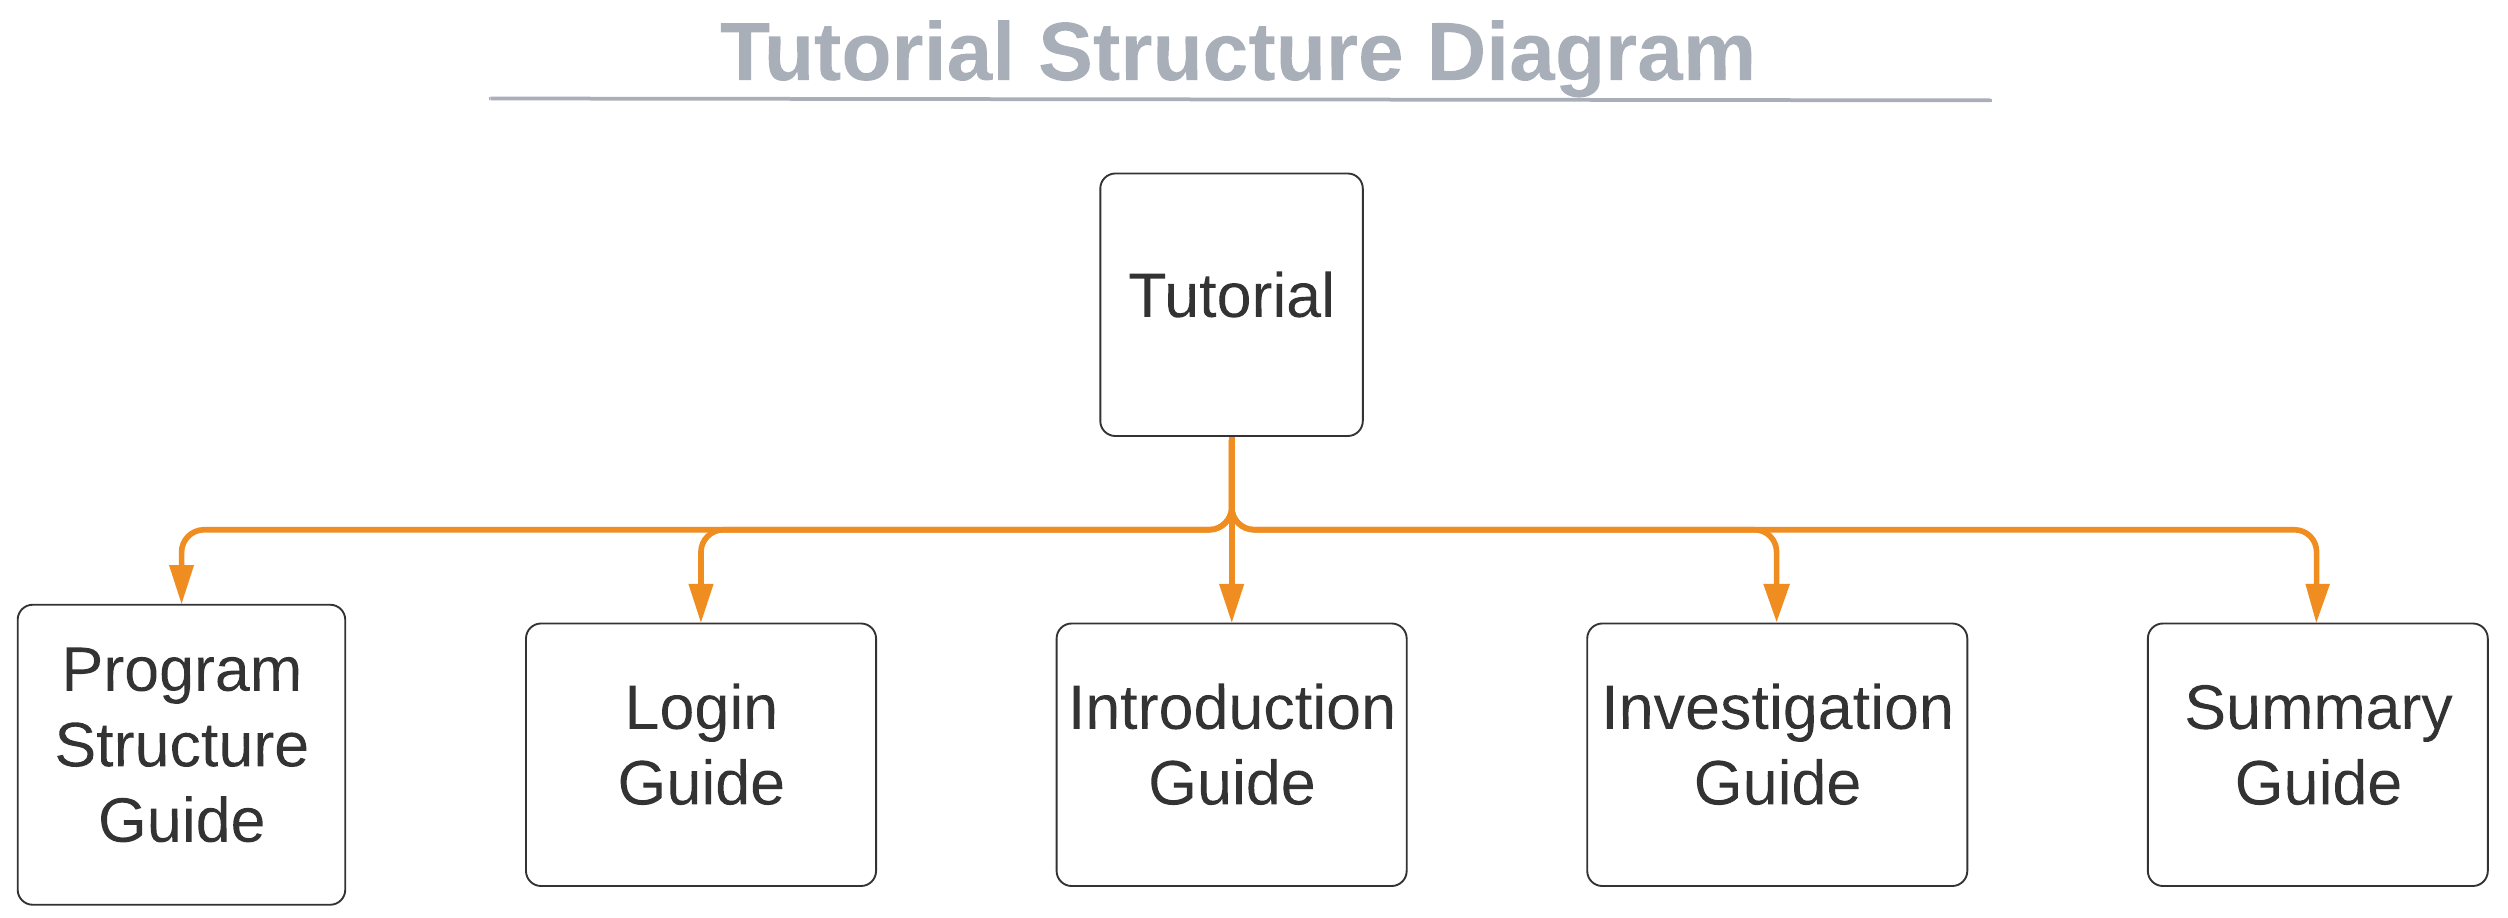
\includegraphics[scale=0.55]{tutorial-structure-diagram}
    \caption{Tutorial Structure Diagram}
\end{figure}

The tutorial itself will be split up into 4 main parts; that is a guide on the structure of the program, and how to use each of the individual sections of the program.

Overall, the tutorial will be relatively simple, and will just give the user an understanding of how to use the program

The Program Structure Guide will inform the user of the layout of the project, and how each section is related to another. It will tell the user how to navigate pages, and how to use key features of the program that will require user input.

Next in the tutorial, will be the Login Guide. This will essentially just be a quick note to the user, about how to sign up and create a strong and complicated password, what to do if you forget your password, or want to change it; as well as explain why the user may or may not want to create an account, and how the program differs whether the user is signed in or not.

As for the Introduction Guide, it will show an example of what the introduction section will look like, and have labels to show how to navigate pages as well as what everything means.

Probably the most complex part of the tutorial section will be the Investigation section. This will inform the user of how to use, understand, and interpret the different graphs and plots. This section should give the user a simple understanding of how they can use the program to investigate the Riemann Hypothesis

The final section in the tutorial will be a Summary Guide, that is how to use the summary section of the program. This will be very similar to the Introduction Guide, but will have an emphasis on the user trying to draw conclusions from the data they have collected, instead of the just being able to understand what is going on.

The tutorial section will not have a lot of functionality, but its purpose is just to briefly describe to the user, how the program is intended to be used.

\clearpage

\subsubsection{Introduction Structure Diagram}
In the Introduction section of the program, the user will be able to develop their understanding of what the Riemann Hypothesis is and why its so important.

I will portray this information by splitting the Introduction into three smaller sections. You can see how this section will be split up in the Structure Diagram below:

\begin{figure}[h]
    \centering
    \captionsetup{justification=centering}
    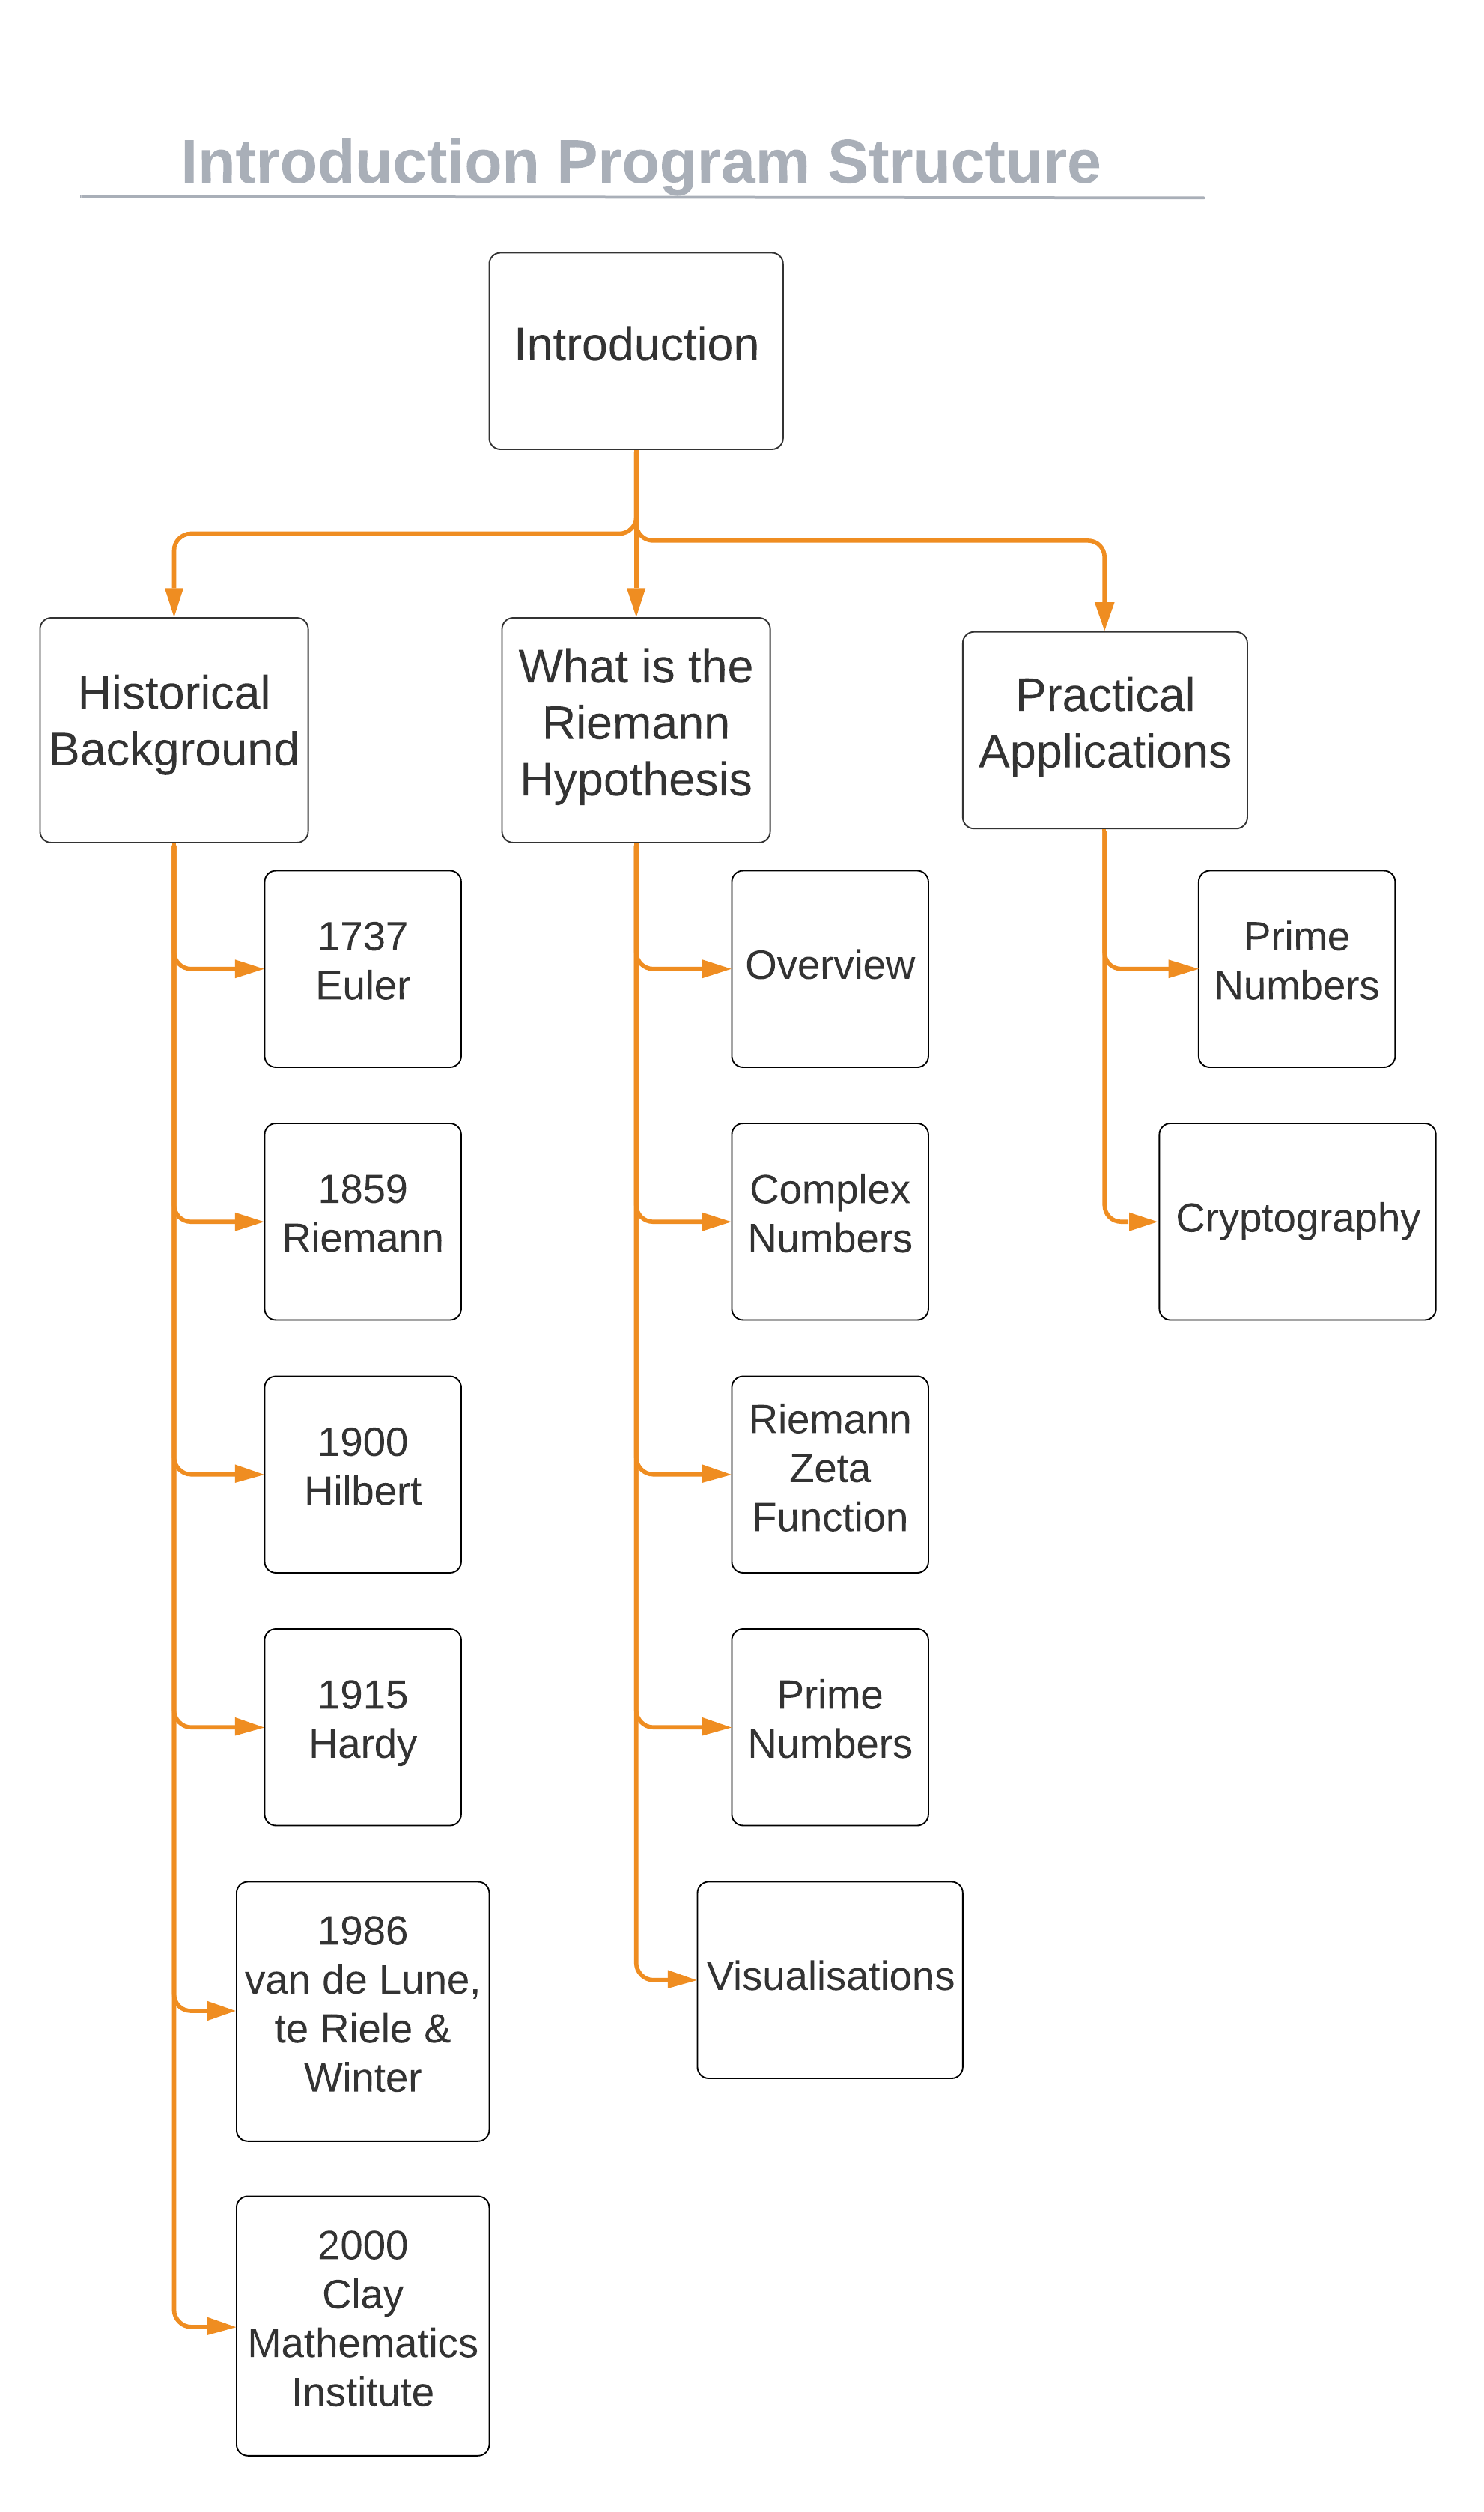
\includegraphics[scale=0.385]{introduction-structure-diagram}
    \caption{Introduction Structure Diagram}
\end{figure}

First of all is the historical background section. This shows how the Riemann Hypothesis has developed over time and showcases the context of the problem

Next is the section describing the Riemann Hypothesis. This section will include a lot of maths, but will also br written such that people will a limited mathematical understanding will still be able to understand what is being said.

The final part of the introduction is the Practical Applications section. This will inform the user why the Riemann Hypothesis affects us today and how it can actually be used.

\clearpage
\subsubsection{Investigation Structure Diagram}
The Investigation is the main part of the program and will allow the user to conduct their own research into the Riemann Hypothesis.

It will have 4 main section; The graphs, Prime Numbers, a zeta function calculator, and a zeta zeros calculator.

\begin{figure}[h]
    \centering
    \captionsetup{justification=centering}
    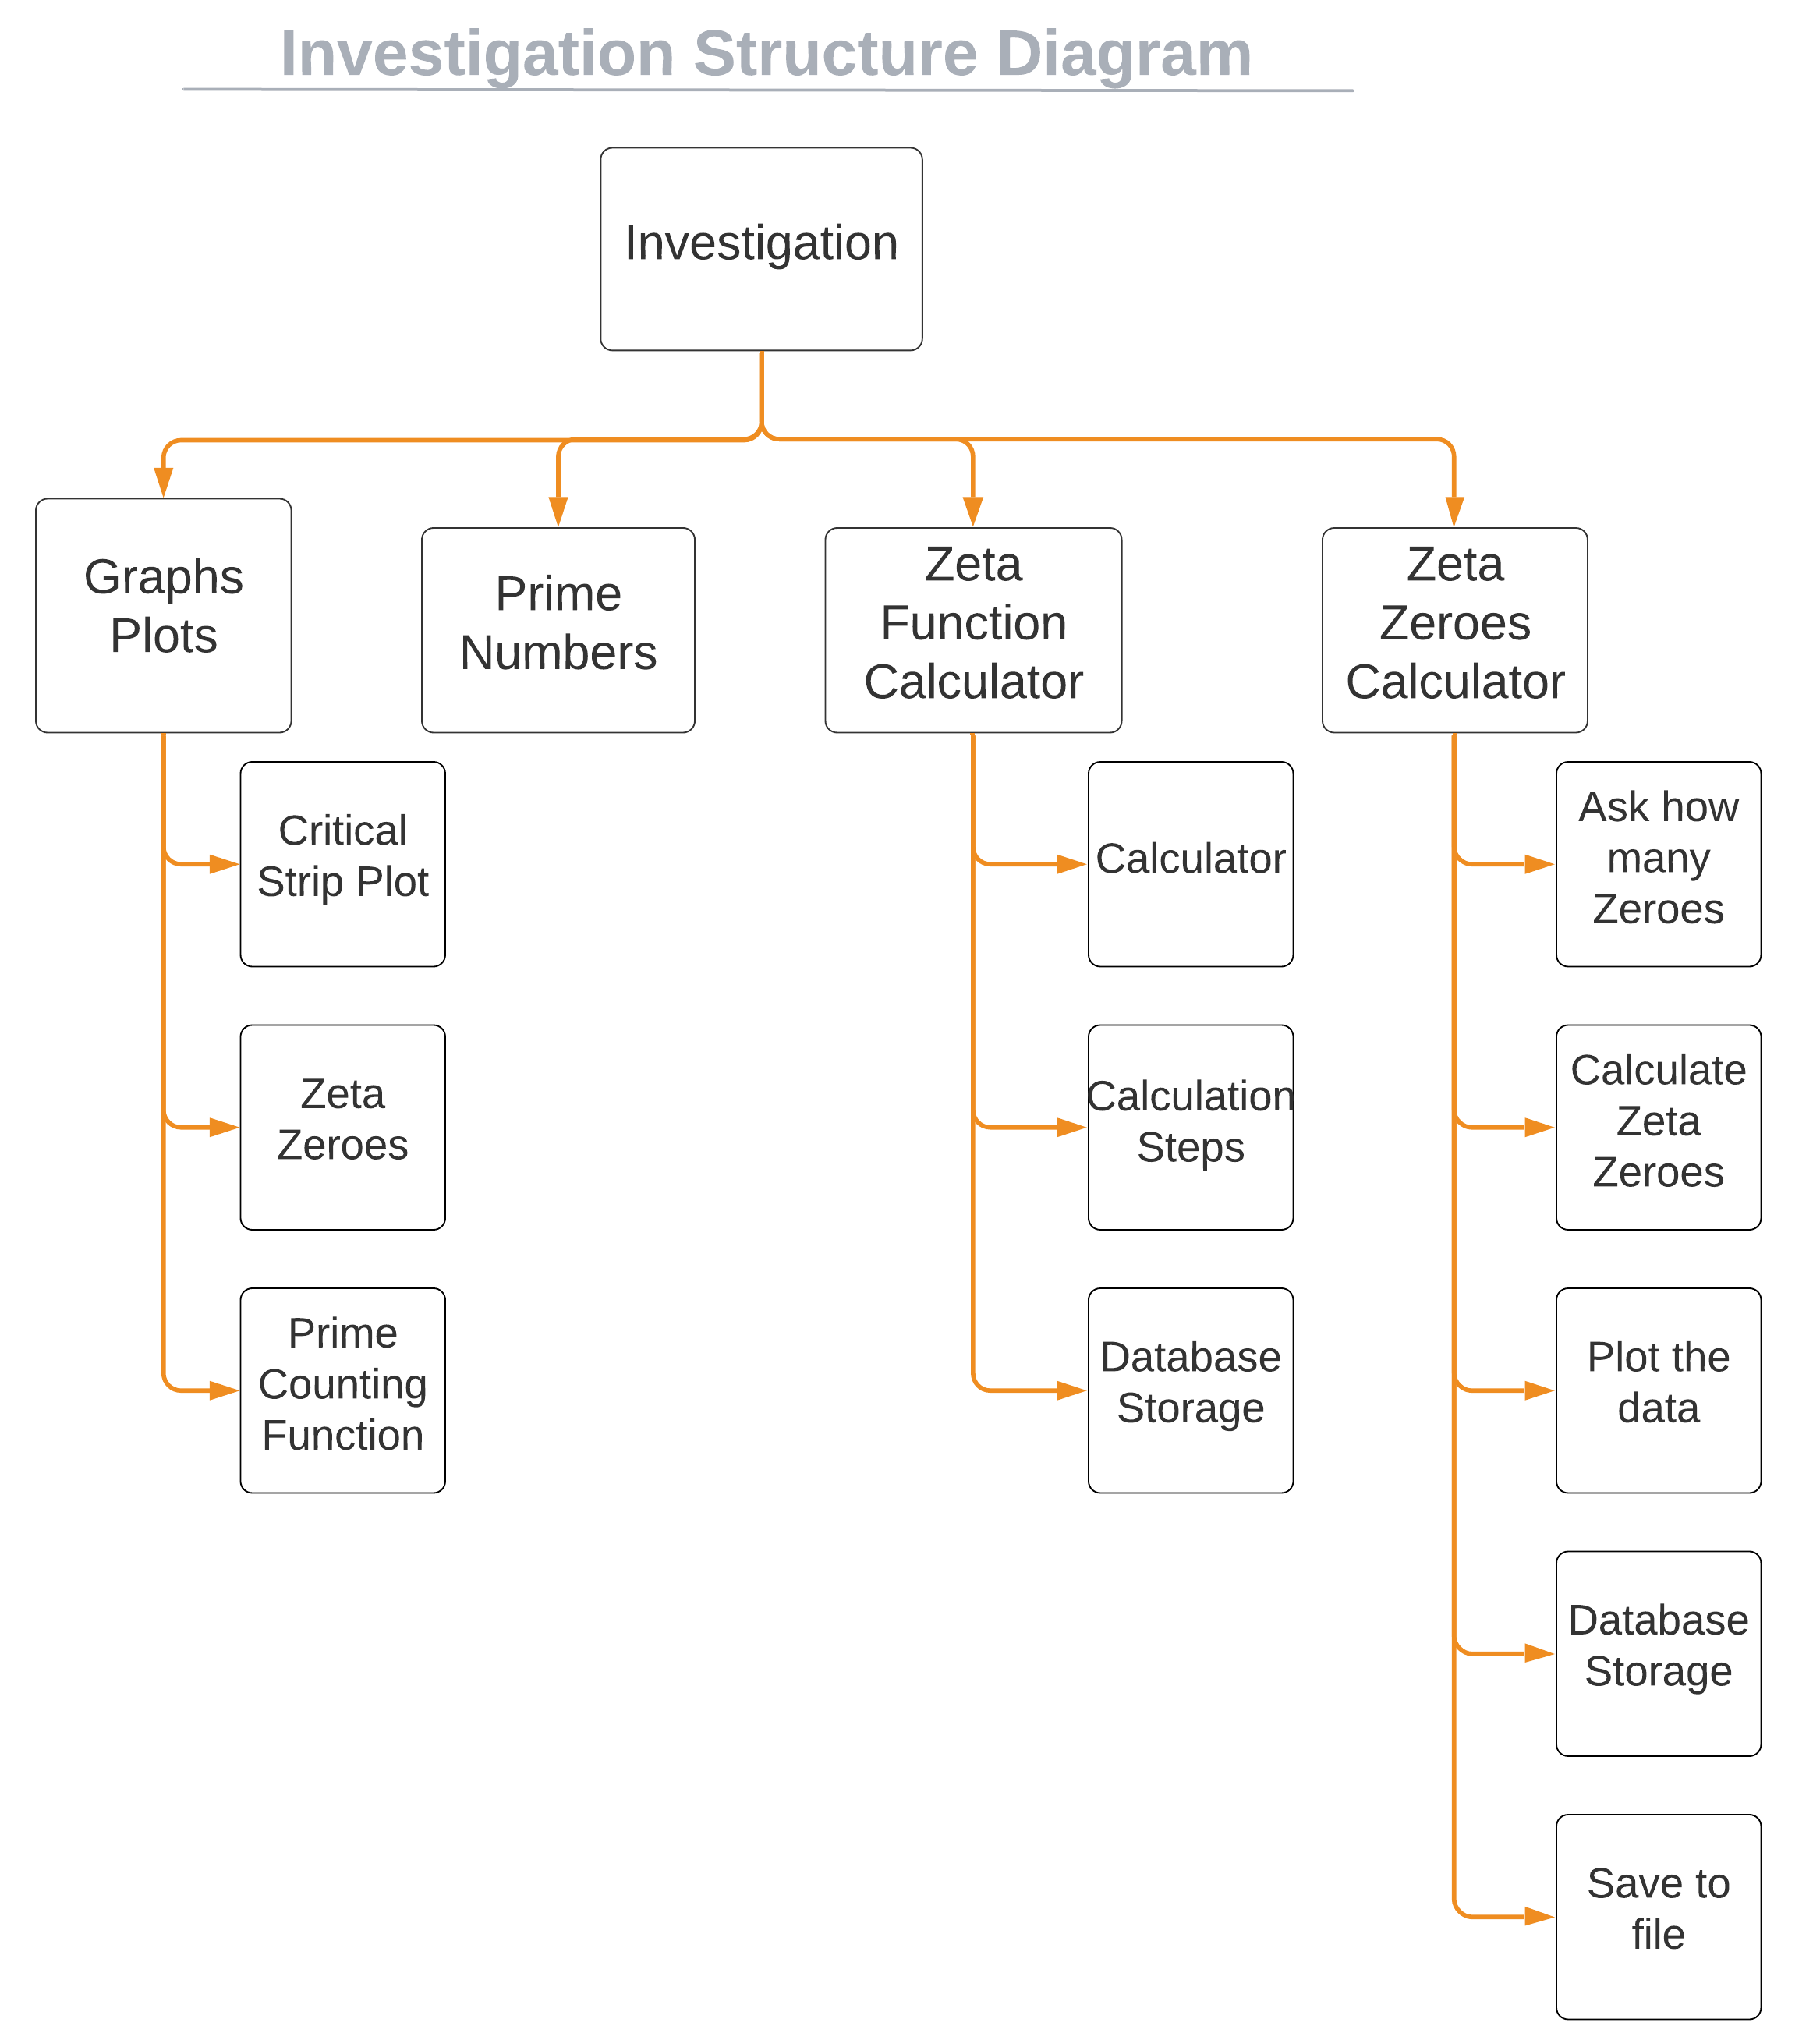
\includegraphics[scale=0.5]{investigation-structure-diagram}
    \caption{Introduction Structure Diagram}
\end{figure}

The first section will be the Graph Plot section. The aim of this section is to display to the user various graph plots that are related to the zeta function. This user will be able to change given inputs into the graph plots and be able to see the output visually.

The prime number section will show the user the correlation between the Riemann Zeta Function and the prime numbers. This section will showcase various graphs and mathematical functions for the user to explore.

Next is the zeta function calculator. This will be a relatively simple part of the investigation section. It will allow the user to input a number (or range of numbers)into the calculator. It then calculates these values and will allow the user to store the data, either in a file or database.

Finally is the zeta zeroes calculator. This will calculate all of the zeta zeroes between two points given by the user, and with accuracy determined by the user. Similarly to the zeta function calculator, the user will also be able to store this data to a database or file, or even display the data in a graph plot.


\subsubsection{Summary Structure Diagram}

The final main section in the program will be the summary. It will be a recap of what the user should have learnt from using the program, and what to take away from it. It will be split up into a theory recap section, a results section, a conclusion and evaluation section and a section on the impact of the Riemann Hypothesis.


\begin{figure}[h]
    \centering
    \captionsetup{justification=centering}
    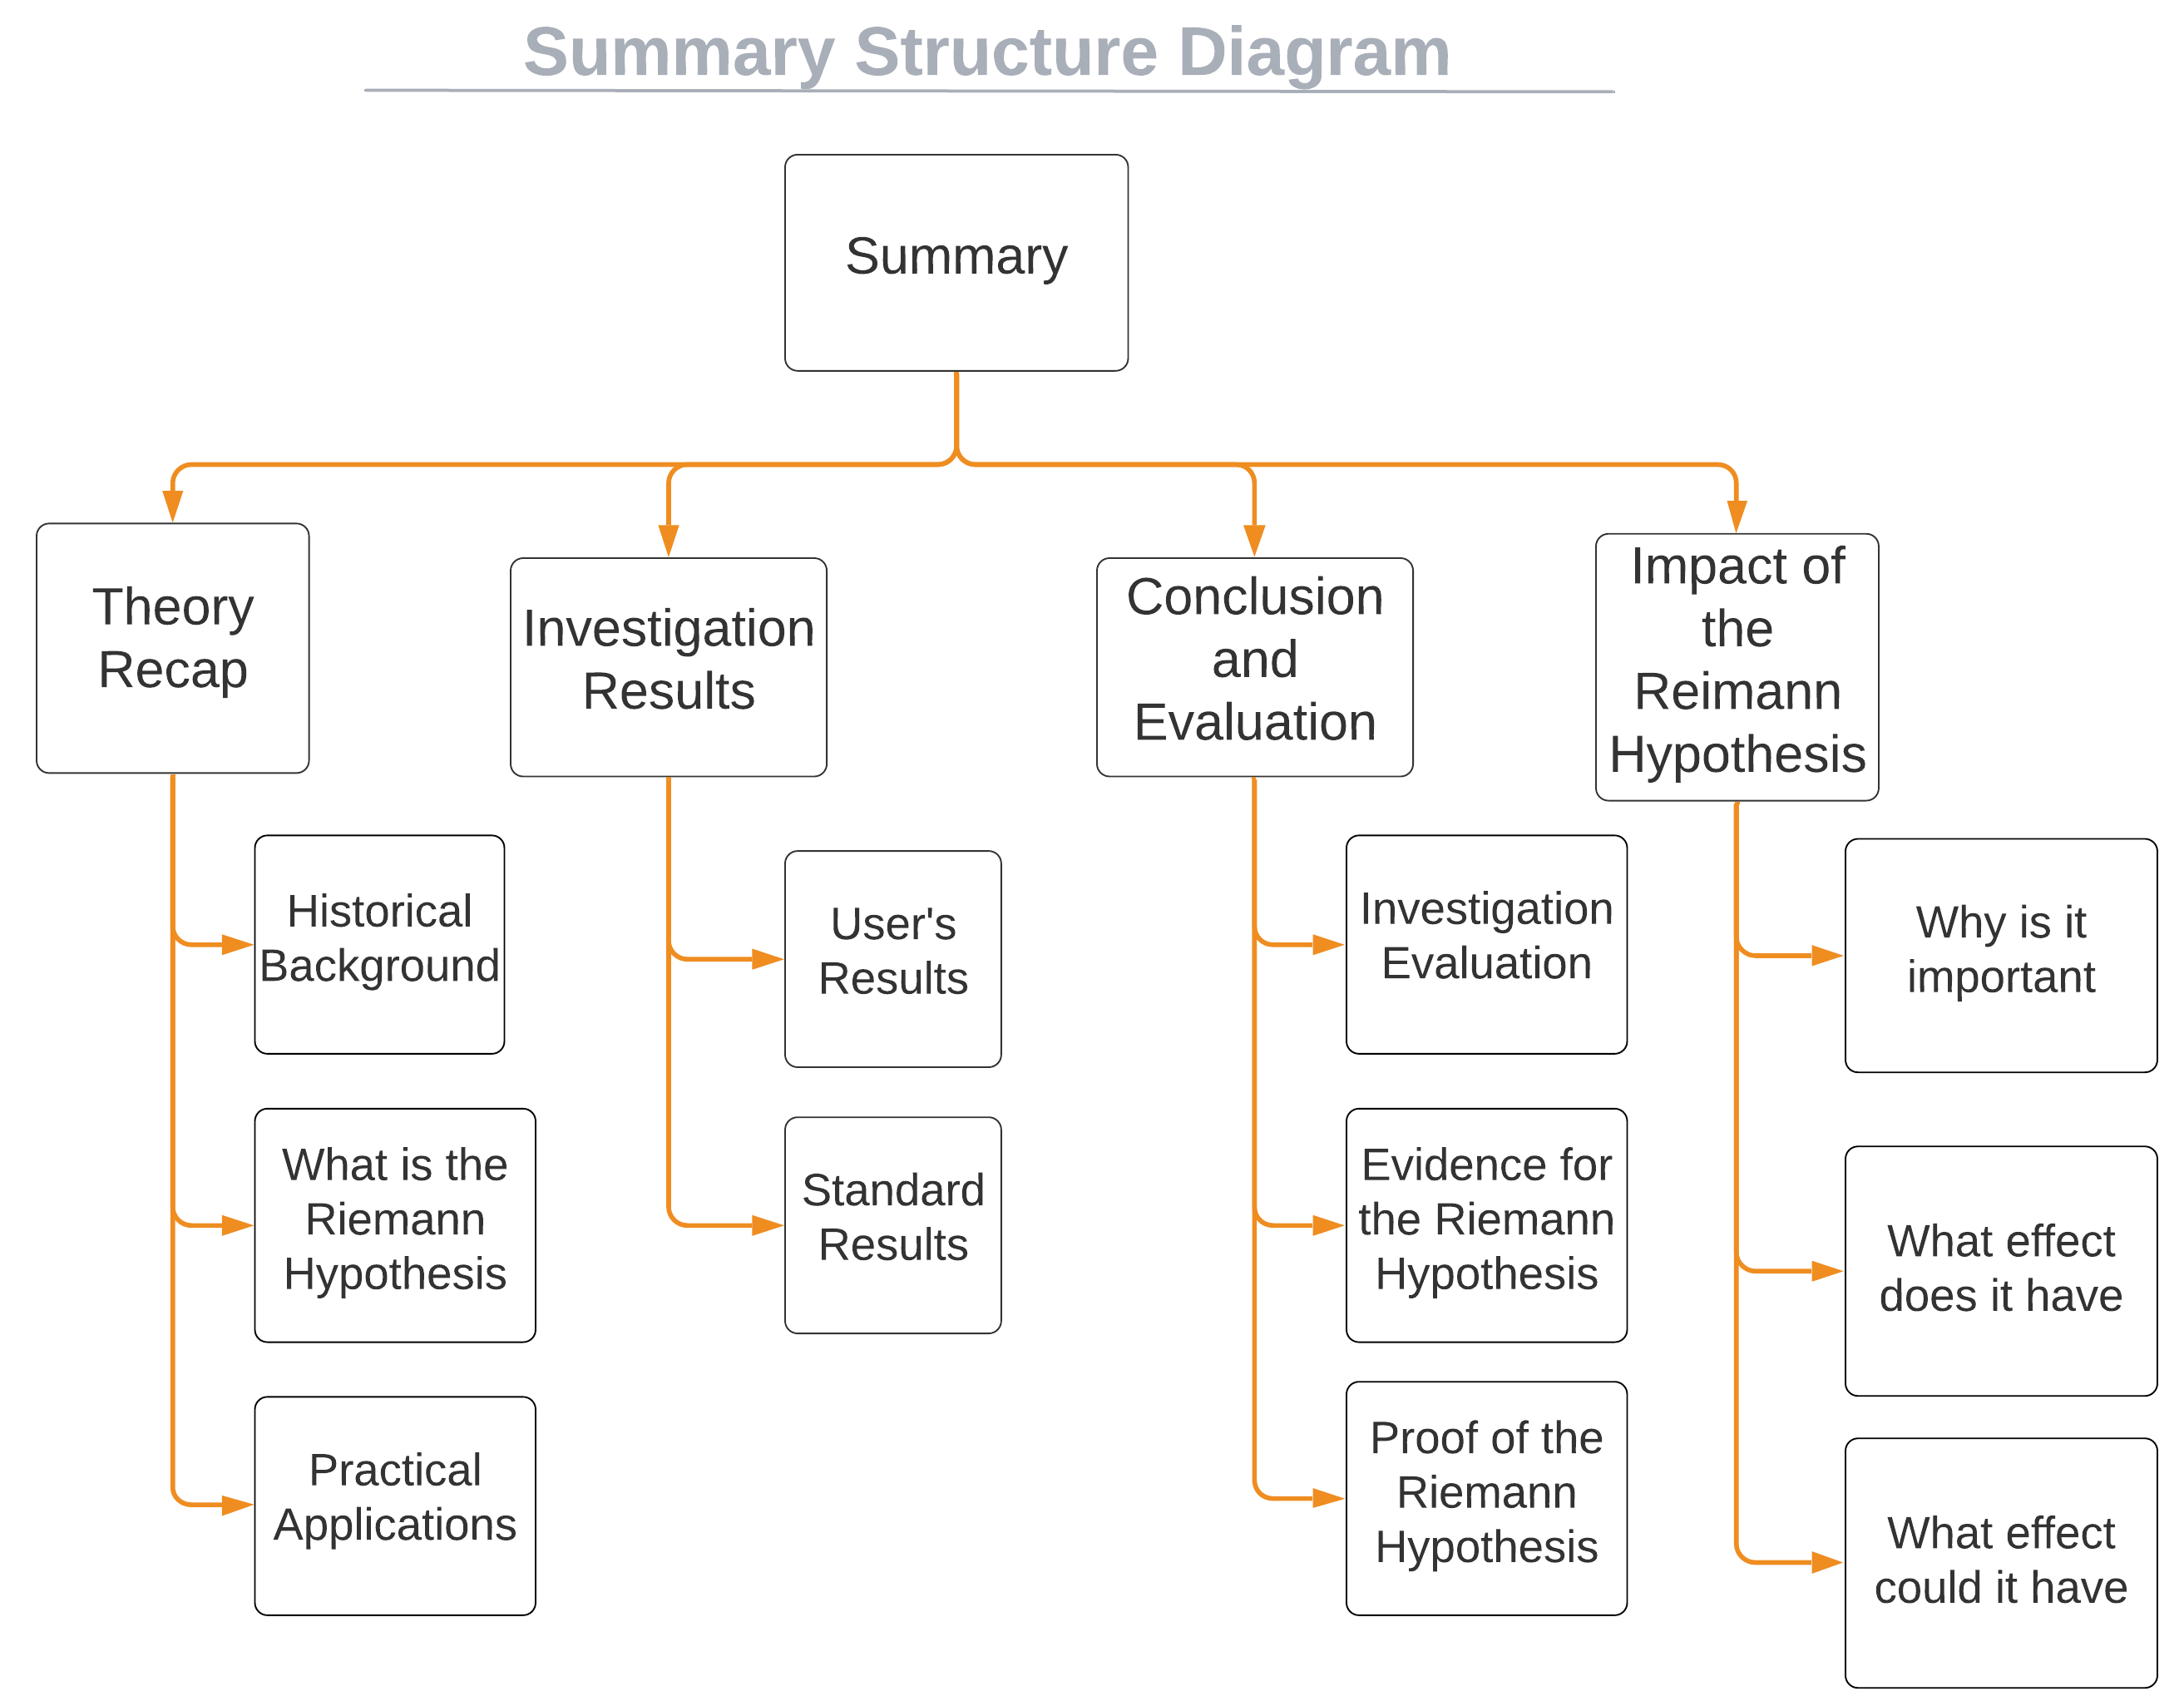
\includegraphics[scale=0.5]{summary-structure-diagram}
    \caption{Summary Structure Diagram}
\end{figure}

The first part of the summary; the theory recap will essentially be a very cut down version of the introduction section. It will provide an overview of the problem such that the user can refresh their mind as to what the Riemann Hypothesis actually is.

As for the investigation results, this page aims to provide the results of the user's investigation. It will provide raw data as well as some visual aids such as graphs. It will also compare the data collected by the user with the expected data.

Next is the conclusion and evaluation section. This section will detail to the user how accurate their results were to the true values, as well as any evidence and proof of the Riemann Hypothesis.

Finally, is the Impact of the Riemann Hypothesis. The aim of this section is to explain to the user why the Riemann Hypothesis is so important by explaining how it affects us.


Overall, I feel as if I have sufficiently broken down my project into a number of more manageable parts that will comes together neatly to form the whole system.
\subsection{Hierarchy Diagrams}

\subsection{System Flowcharts}

\subsection{Data Flow Diagrams}

\clearpage
\subsection{Object-Oriented Design}
\begin{figure}[h]
    \centering
    \captionsetup{justification=centering}
    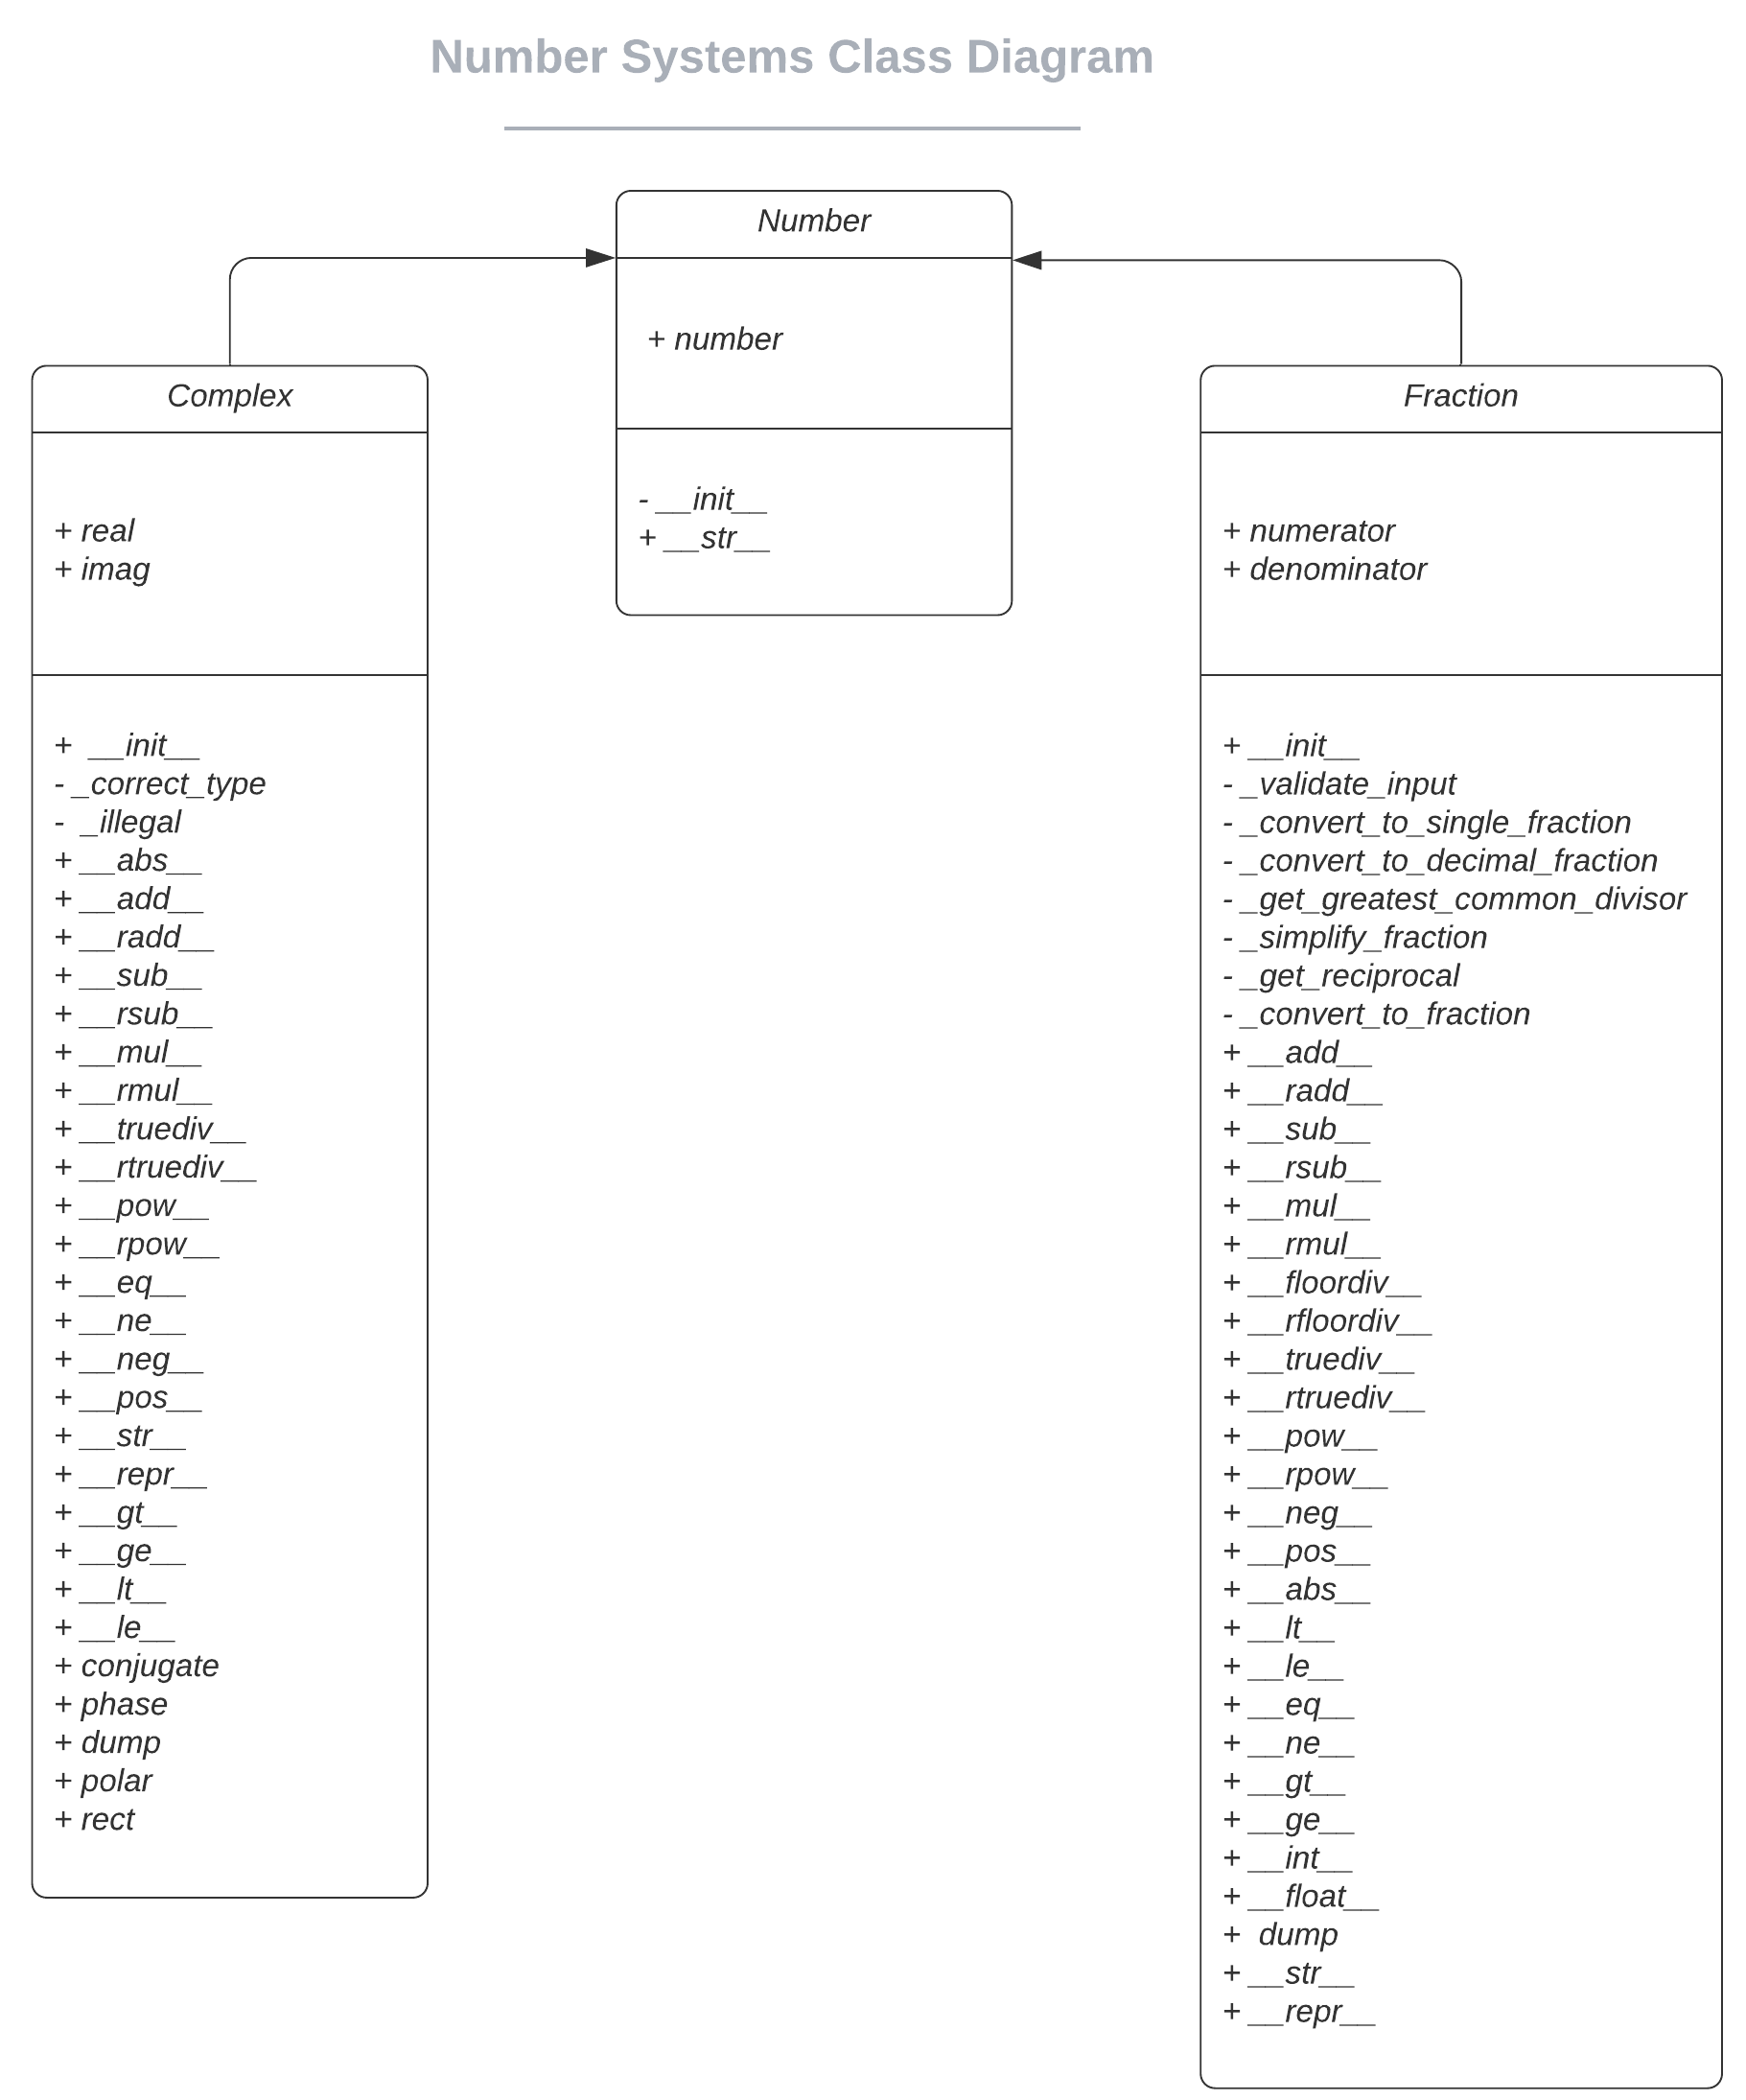
\includegraphics[scale=0.6]{number-systems-class-diagram}
    \caption{Number Systems Class Diagram}
\end{figure}
As part of this project I will need to be able to represent many types of numbers namely, fractions and complex numbers. The best way to do this is to use Classes and Object-Oriented Programming. I can create a data structure in python, such that they will be able to store all of the necessary data, and perform all the operations that I need.

All of the data types will inherit attributes and methods from a main \textit{‘Number’} Class. This number class will have basic attributes and methods, allowing a number to be defined and printed.

The complex number class is a lot more substantial than the number class.  It will allow for inputs in Rect form, or Modulus Argument Form. The methods in this class will allow for the user to add, subtract, multiply, divide, and use exponentials with complex numbers. There will also be a set of private functions in the class in order to change between cartesian and polar form.

As for the fraction class, it will take inputs of a numerator and denominator, and will allow the user to use public functions in order to perform operations and calculations involving fractions.

These classes will be able to let me sufficiently perform precise calculations with numbers. The fraction class removes any mathematical floating point errors from calculations, and the complex class will allow me to utilise imaginary and complex numbers in Python.

Some points to note; I have tailored this class diagram and the following pseudocode for a Python programme. Conventionally, when calling a function prefix notation is used. For example, if we have a simple function as follows:

\begin{algorithm}
    \caption{Prefix add function}
    \begin{algorithmic}
        \Function{add}{$a$, $b$}\\
             \hspace{\algorithmicindent}\Return $a + b$
        \EndFunction
    \end{algorithmic}
\end{algorithm}

Then we can see that it takes two inputs, a and b, and will return their sum.

To call this function, we will use prefix, notation with the function name at the beginning, followed by the two parameters.
Such as:

\begin{algorithm}
    \caption{Calling the prefix add function}
    \begin{algorithmic}
       \State \Call{add}{$a$, $b$}
    \end{algorithmic}
\end{algorithm}

However, in Python, we are able to create mathematical functions that allow for infix notation. This is a more natural way of calling maths functions. To allow for infix notation, we add two underscores to the beginning and end of the function name when we define it. So for some example python code:


\begin{lstlisting}
# Python infix add function
def __add__(a, b):
    return a + b
\end{lstlisting}

We can run it by calling

\begin{lstlisting}
# Python call infix add function
    a = 1
    b = 2
    c = a + b
\end{lstlisting}

Which is infix notation. Now in this example, it may seem almost obsolete to create a function that already mimics the behaviour of what we are trying to achieve, however using this notation we are able to overwrite the existing infix notation in python, and even create new notation of any data types that we choose to create.

A simple example of this is with the fraction class. There is no inbuilt class for handling fractions in python, so we can create one and allow it to use infix notation.

If we have a fraction class that takes a numerator and denominator as an input, and have this function defined in the class, it would look as follows:


\begin{lstlisting}
# Python __add__ as part of the Fraction Class
def __add__(self, other):
        """ self + other """
        other = self._convert_to_fraction(other, 'addition')
        resulting_numerator = self.numerator * other.denominator +
                              self.denominator * other.numerator
        resulting_denominator = self.denominator * other.denominator
        return (Fraction(resulting_numerator, resulting_denominator))
\end{lstlisting}

This function finds a common denominator for the fractions and then adds the numerators together.

To call this function to add $\frac{3}{4}$ and $\frac{1}{2}$ , we would use infix notation as follows:


\begin{lstlisting}
# Python calling __add__ for two instances of the class Fraction
Fraction(3, 4) + Fraction(1, 2)
\end{lstlisting}

Which would return the correct value of $\frac{5}{4}$.

As we can see from this example, we have created a python function that can be called using infix notation, rather than the standard postfix notation.

One other point to note is that python does not handle infix notation for user defined data types very well. If we want to compute the user defined \textit{Fraction} + the Python Integer $3$, this is okay. But due to the way python has been created, we would be unable to do Integer $3$ + \textit{Fraction}. For this we need to define another function called \textit{\_\_radd\_\_}, short for right add. This allows us to still compute the infix addition, even when the user defined variable is on the right hand side of the addition sign. The \textit{\_\_radd\_\_} function would use the already created \textit{\_\_add\_\_} function, but would have its arguments swapped and the code would look as follows:

\begin{lstlisting}
# Python infix radd function
def __radd__(self, other):
        """ other + self """
        return self.__add__(other)
\end{lstlisting}

This would swap the arguments around so that the \textit{\_\_add\_\_} function is then called with the parameters in the correct position.

\clearpage
\subsection{Database Design}
\clearpage

\subsection{Key Algorithms Design}
Throughout this section, I will be modelling some of the key algorithms used throughout this project. For each algorithm, I will describe how it works using structured English, represent it by using a flowchart, and then write the algorithm in Pseudocode and Python.

\subsubsection{Euclidean Algorithm}
The Euclidean Algorithm is a method for computing the greatest common divisor of two integers. The greatest common divisor is the largest number that divides into both of the numbers without a remainder. This algorithm is recursive.

It works by, first, taking in two integers $a$ and $b$. These are the numbers for which the greatest common divisor will be found. I will explain how this algorithm works through the use of an example.

Say we want to find the greatest common divisor of 45 and 10.
We would first take the largest of the two numbers, and set that equal to some multiple of the smaller number, plus some remainder.
$$45 = 10 \cdot n + r$$
Where $n$ is the multiple of the smaller number, and $r$ is the remainder.
We can then compute what the values of $n$ and $r$ are. For this example, $n = 4$ and $r = 5$.
$$45 = 10 \cdot 4 + 5$$
Say we then use this as a general equation
$$a = b \cdot n + r$$
The next step (and every other step) of the algorithm is to take the value of $b$ and move it to the left hand side of the equation, replacing the value of $a$. We then do a similar thing by replacing the value of $n$ with the value of $r$. This process is repeated until $r = 0$.

Completing this step would look as follows:
$$10 = 5 \cdot n + r$$
Then working out the values of $n$ and $r$
$$10 = 5 \cdot 2 + 0$$
And now the repeating process stops because $r=0$. We then output the value of $b$, and that is the answer for the greatest common divisor of the two numbers $a$ and $b$. So for this example, the greatest common divisor of $45$ and $10$ is $5$.

Now, lets see how this algorithm works on a larger example, where we want to work out the greatest common divisor of $300$ and $245$.
$$300 = 245 \cdot n + r$$
$$300 = 245 \cdot 1 + 55$$
$$245 = 55 \cdot n + r$$
$$245 = 55 \cdot 4 + 25$$
$$25 = 5 \cdot n + r$$
$$25 = 5 \cdot 5 + 0$$

Then our answer is the value at position $b$ in $a = b \cdot n + r$, which is $5$. So the greatest common divisor of $300$ and $245$ is 5.

Now, earlier I mentioned that we start by taking the larger of the two inputs, and place that on the left hand side of the equation, but really, the algorithm works no matter which input starts on the right of the equation. Say instead of calculating the greatest common divisor of $300$ and $245$, we want to calculate the greatest common divisor of $245$ and $300$. We would start by forming the equation:
$$245 = 300 \cdot n + r$$
And then working out the values of $n$ and $r$:
$$245 = 300 \cdot 0 + 245$$
For any set of values where the smaller input is at position $a$, we will always be left with $n = 0$ and $r = a$.

Following through with the algorithm, the next step would be:
$$300 = 245 \cdot n + r$$
This is exactly how we started the previous example. This shows that it doesn't matter which way round the two input numbers go in the algorithm, it will always compute the same number.

In other words, the greatest common divisor of $a$ and $b$, is the same as the greatest common divisor of $b$ and $a$, which intuitively makes sense.
\clearpage
Now using flowcharts, we can write the algorithm as follows:

\begin{figure}[h]
    \centering
    \caption{Euclidean Algorithm Flowchart}
    \captionsetup{justification=centering}
    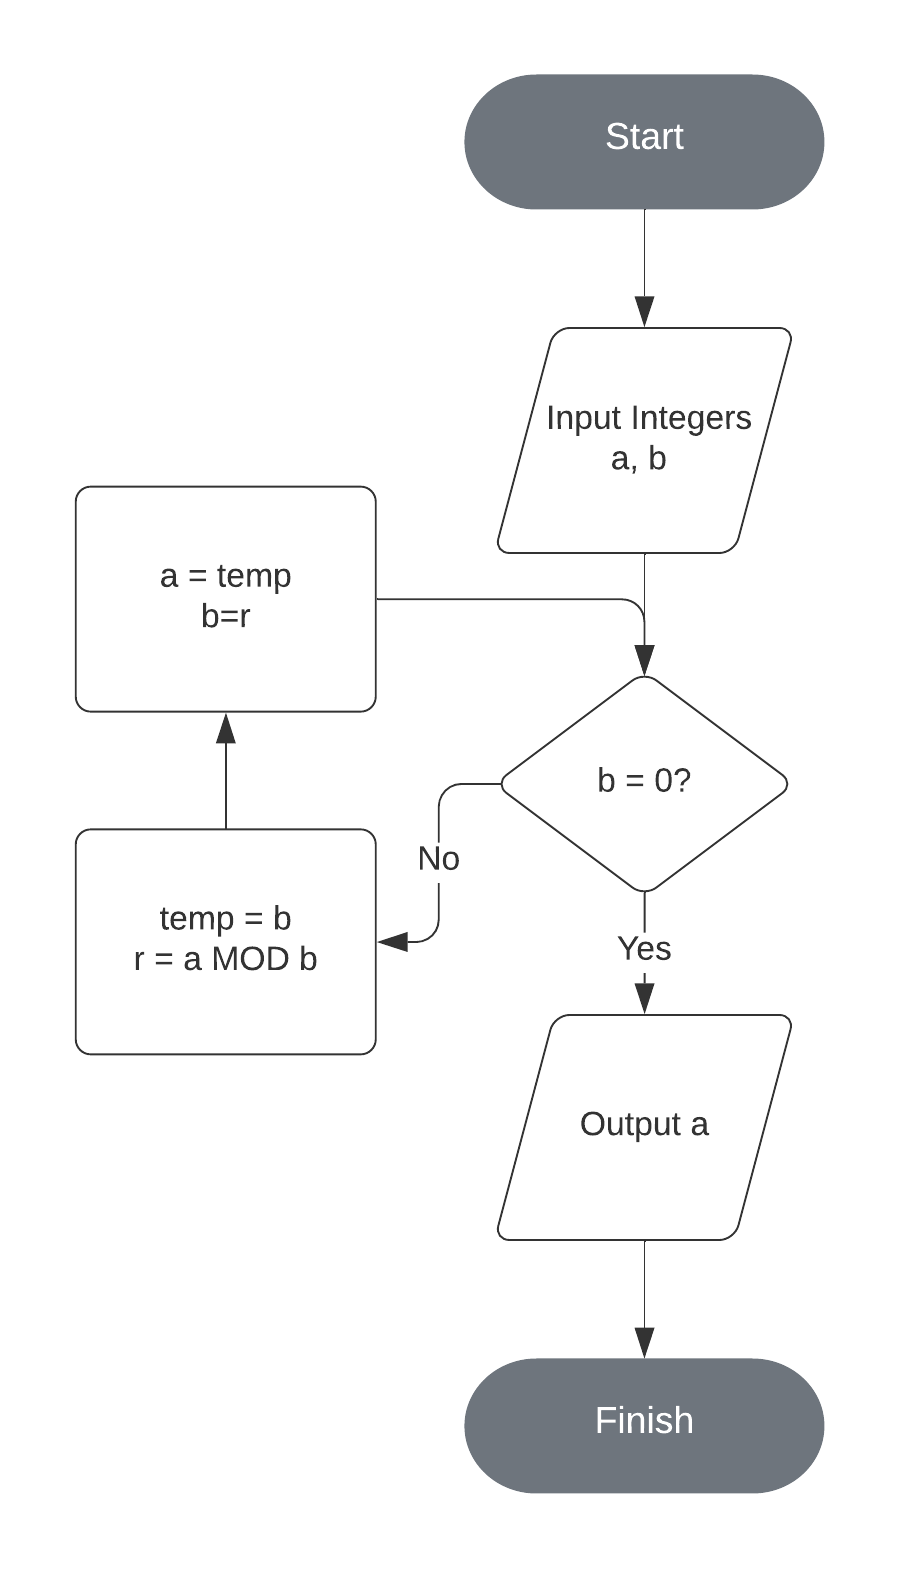
\includegraphics[scale=0.6]{euclidean-algorithm-flowchart}
\end{figure}

By representing the algorithm as a flowchart, we can see that it starts of by receiving two integers $a$ and $b$ as an input, and then keeps on finding the values of $n$ and $r$ from the examples, until the value of $b$ is $0$. Implementing this as code, this looping could be done using a standard \texttt{WHILE} loop, but I think that implementing this algorithm as a recursive function would be more suitable.

Implementing this algorithm in pseudocode, it would look as follows:
\begin{algorithm}
    \caption{Euclidean Algorithm Pseudocode}
    \begin{algorithmic}
        \Function{greatest\_common\_divisor}{a, b}
            \If {$b = 0$}
                \State \Return $a$
            \Else
                \State\Return\Call{greatest\_common\_divisor}{$b$, $a$ MOD $b$}
                \Comment{recursively call the function until $b = 0$}
            \EndIf
        \EndFunction
    \end{algorithmic}
\end{algorithm}

We can see from this pseudocode, the recursive nature of this algorithm.
\clearpage
Then writing the Euclidean Algorithm in Python:

\begin{lstlisting}
# Euclidean Algorithm
def greatest_common_divisor(a: int, b: int) -> int:
    if b == 0:
        return a
    else:
        # recursively call the function until b = 0
        return greatest_common_divisor(b, a % b)
\end{lstlisting}

This implementation of the Euclidean Algorithm in Python, is very efficient. Although it is recursive, and that can in some circumstances lead to a large amount of memory use - especially in Python - it would be relatively simple to unwind the stack at the end of the computation, because this function does not call any other functions and is relatively simple.


\subsubsection{Riemann Zeta Function}
One of the most important mathematical functions in this project is the Riemann Zeta Function. As mentioned in my analysis section, it can be defined as:
% \begin{align*}
    $$\zeta(s) = \sum^{\infty}_{n=1}\frac{1}{s^n}$$
Which can be rewritten as:
    $$\zeta(s) = \frac{1}{1-2^{1-s}} \sum_{n=0}^{\infty} \frac{1}{2^{n+1}} \sum_{k=0}^{n} (-1)^k \binom{n}{k} (k+1)^{-s}$$
% \end{align*}

This is just one of many of the ways that $\zeta(s)$ can be defined. The main advantages of this definition are that it is will allow inputs for any complex number $s$ (apart from when $s = 1$ for which $\zeta(s)$ is undefined), and that it is fast to compute.
\clearpage
Using flowcharts, we can write this function as follows:
\begin{figure}[h]
    \centering
    \caption{Zeta Function Flowchart}
    \captionsetup{justification=centering}
    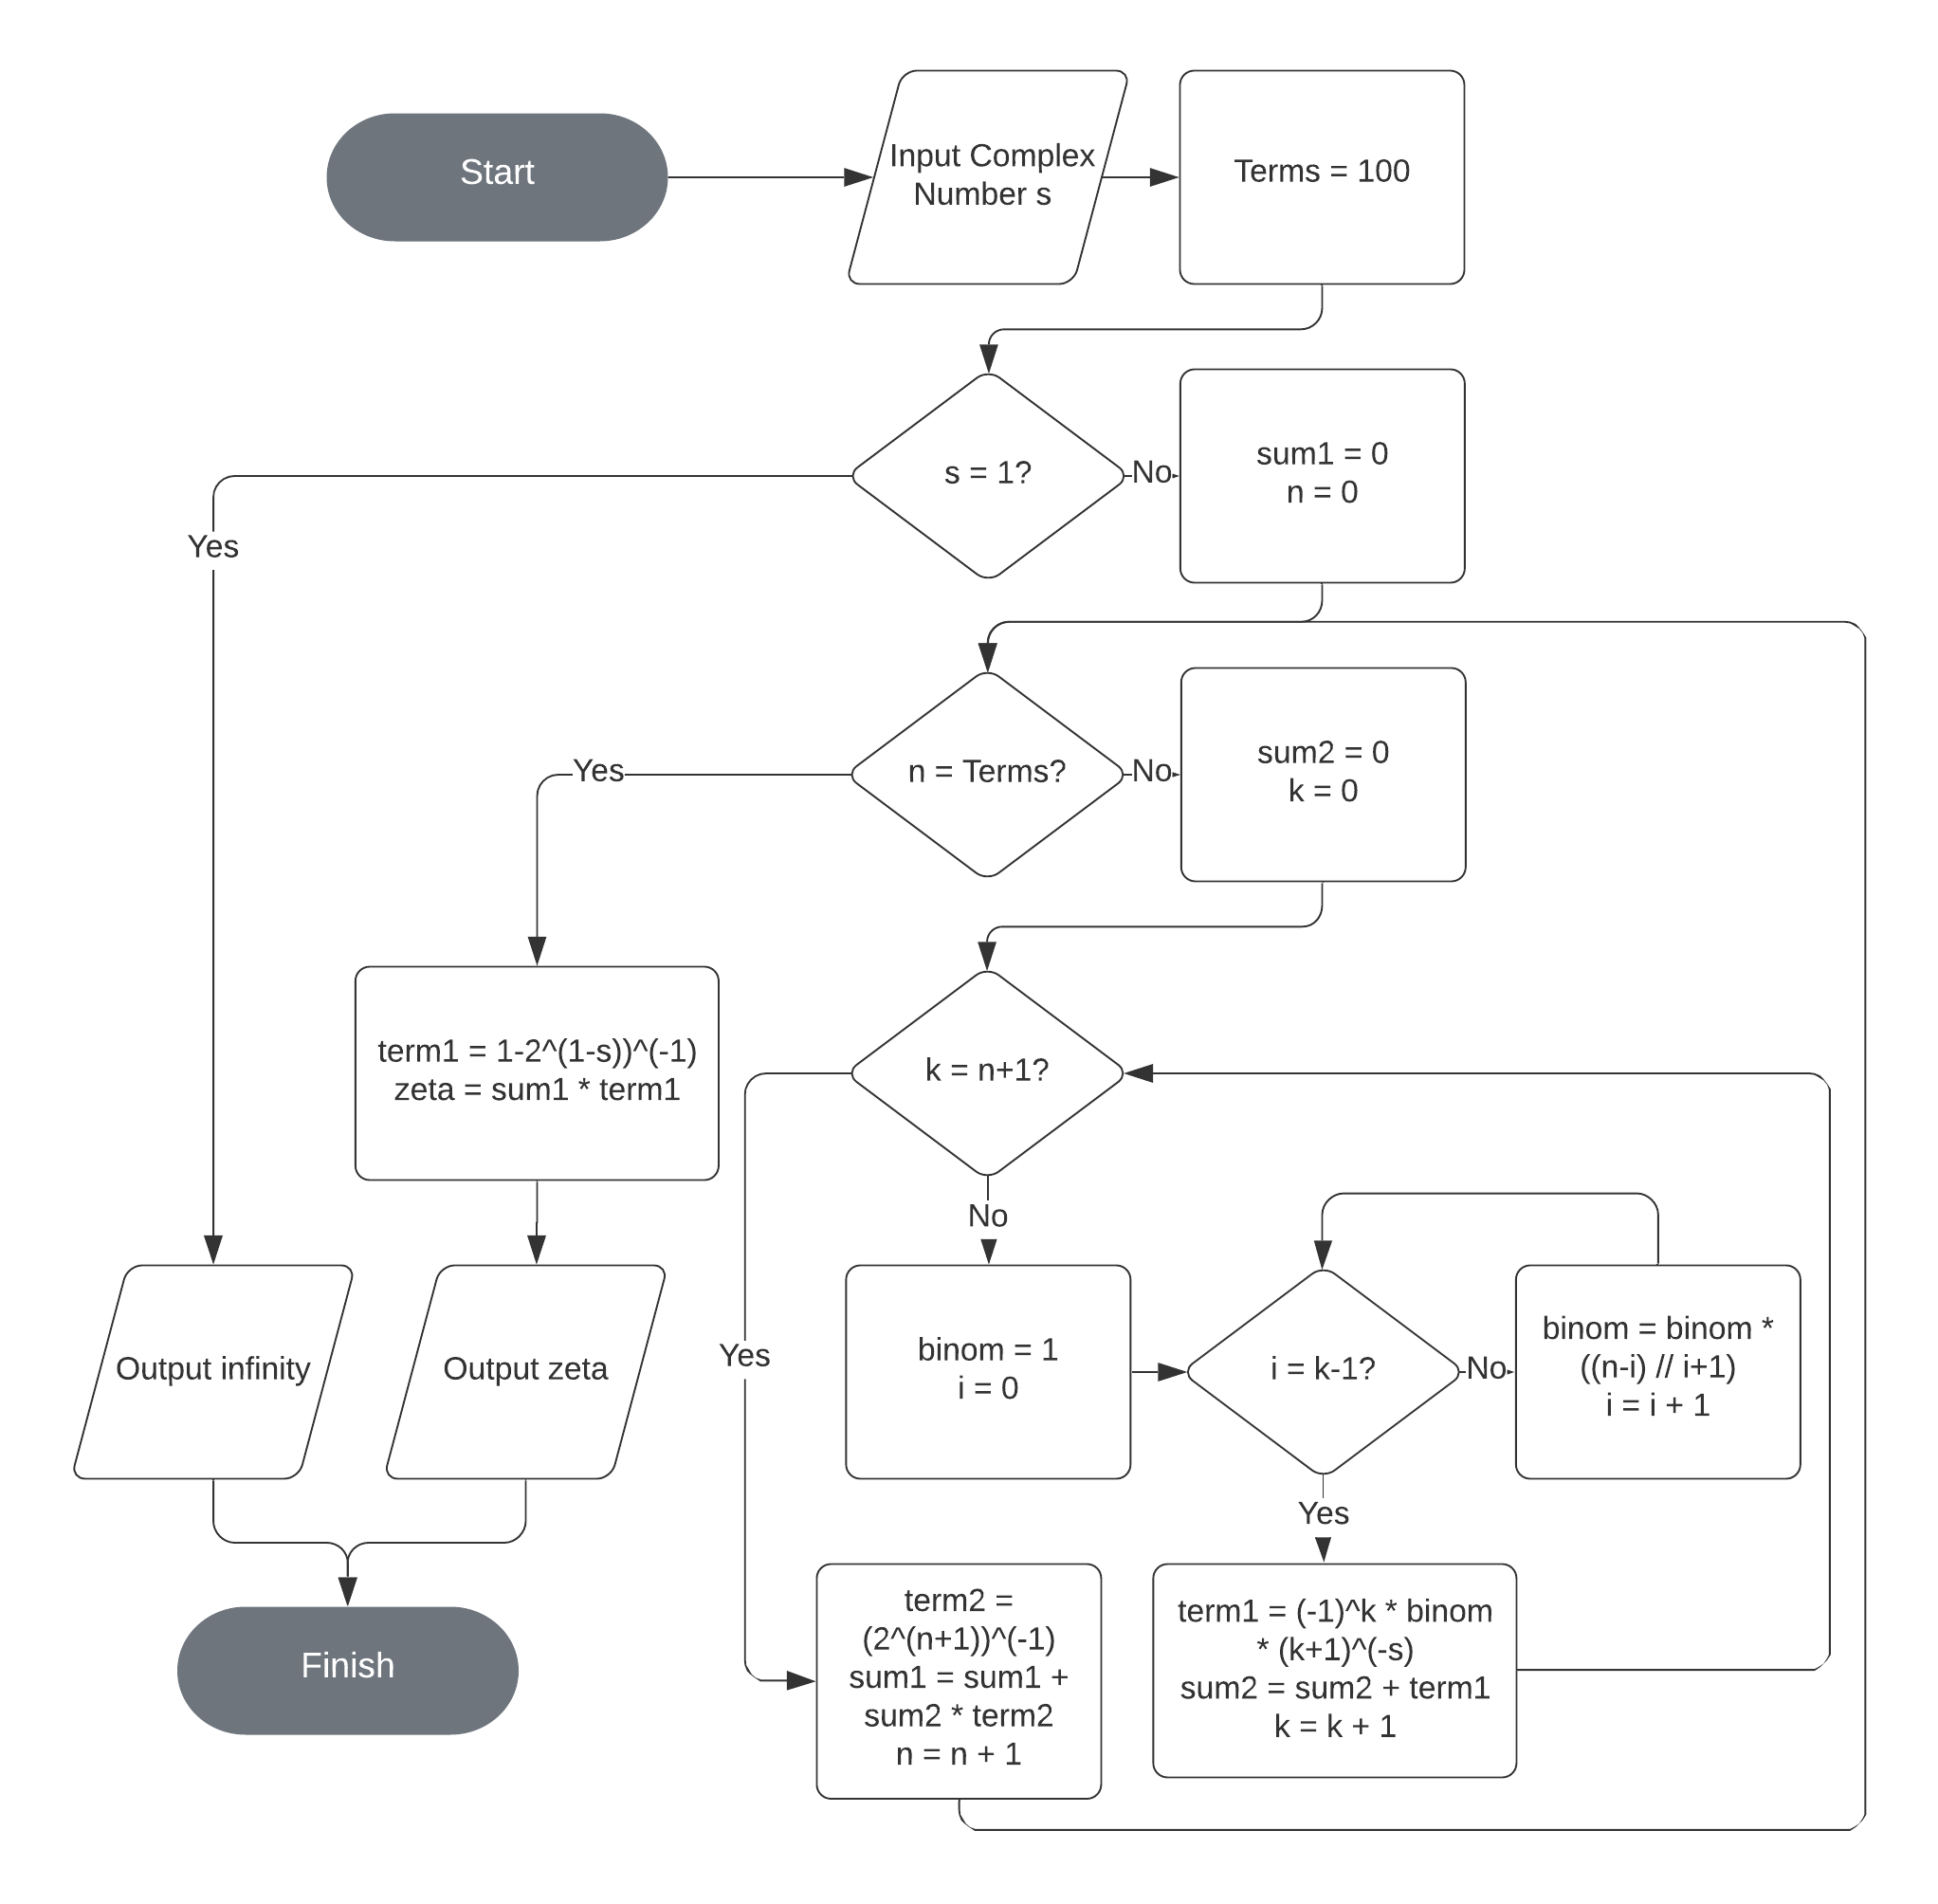
\includegraphics[scale=0.6]{zeta-function-flowchart-two}
\end{figure}

Unfortunately, with any computational implementation of the zeta function, it would be impossible to calculate an exact output for any given input. This is due to the fact that the zeta function, be definition is the sum of an infinite series.

It would be intractable to compute every single element in the series to be able to sum it. Because the infinite sum is convergent (except for $\zeta(1)$ which cannot be calculated), we can approximate the sum by calculating a very large number of terms in the sum, instead of an infinite amount. The number of terms we calculate in the sum is a trade-off between the time it takes to compute the function, and the accuracy of our answer.

This is what the variable \texttt{Terms}, in the flowchart, is used for. Its aim is to replace the $\infty$ in the infinite loop, such that we can still compute $\zeta(s)$ to a high degree of accuracy, with the function still being relatively time efficient.

In a sense, we are changing our definition of the zeta function, so the function that we are actually calculating is this:

$$\zeta(s) \approx \frac{1}{1-2^{1-s}} \sum_{n=0}^{\texttt{Terms}} \frac{1}{2^{n+1}} \sum_{k=0}^{n} (-1)^k \binom{n}{k} (k+1)^{-s} $$

Which is a less accurate version of the zeta function, but is actually computable.

From the flowchart, we can see how the situation where $s=1$ is handled. $\zeta(1)$ is undefined, so we would be unable to calculate this. Therefore, we have to check this special case, and if $s=1$, then the function will \texttt{OUTPUT Infinity}, otherwise, it will just continue with the rest of the function.

The rest of the function, is essentially just creating two sequences and summing them. The flowchart represents this well, it allows us to visualise the looping nature of the sequences.

We can break down our formula for the approximation of $\zeta(s)$, which will make it clear how the flowchart is designed to work.

\begin{figure}[h]
    \centering
    \caption{Decomposed Zeta Function}
    \captionsetup{justification=centering}
    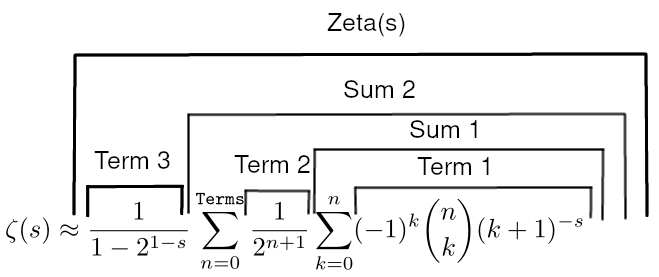
\includegraphics[scale=0.4]{zeta-approx-explained}
\end{figure}

From this image, we can see that:

$$\zeta(s) = \texttt{Term3} \cdot \texttt{Sum2}$$
Where:
$$\texttt{Sum2} = \sum \texttt{Term2} \cdot \texttt{Sum1}$$
Where:
$$\texttt{Sum1} = \sum \texttt{Term1}$$

Then, all that has to be done is replace the values of \texttt{Term1}, \texttt{Term2}, and \texttt{Term3} with their respective values, and that is essentially what is being calculated.

By applying decomposition to the function, we can now easily see how the flowchart works, and now how to implement this function by using pseudocode.
\clearpage
\begin{algorithm}[h]
    \caption{Zeta Function Pseudocode}
    \begin{algorithmic}
        \Function{zeta}{s}
            \State{TERMS = 100}
            \If {$s == 1$}
                \State{ \Return {$\infty$}}
            \Else
                \For {n = 0 \textbf {to} TERMS}
                    \State {sum1 = 0}
                    \For {k = 0 \textbf{to} n+1}
                        \State {sum2 += $(-1)^k \cdot \binom{n}{k} \cdot (k+1)^{-s}$}
                    \EndFor
                    \State{sum1 += sum2 $\cdot \frac{1}{2^{n+1}}$}
                \EndFor
                \State \Return{sum1 $\cdot \frac{1}{1-2^{1-s}}$}
            \EndIf
        \EndFunction
    \end{algorithmic}
\end{algorithm}

For sake of readability, I have omitted creating separate variables for \texttt{Term1}, \texttt{Term2}, and \texttt{Term3}. Instead, these can just be seen by the mathematical equations present in the Pseudocode.

I much prefer this representation of the function, as it easily allows you to see how the sums are implemented alongside the terms. The use of \texttt{for} loops makes it easy to see how we have a sum being calculated inside a sum.

With pseudocode, I have just been able to write the mathematical statements for readability sake, however, when implementing this as a programming language, it could look rather messy with long maths having to be written out.
One area that would need addressing when converting this pseudocode to an actual language is with the binomial coefficient, that is $\binom{n}{k}$. I have previously mentioned this in my analysis, however:

$$\binom{n}{k} = \frac{n!}{k!(n-k)!}$$

Where:
\begin{align*}
    x! &= \prod_{a=1}^x a\\
    &= a \times (a-1) \times (a-2) \times (a-3) \times \dots \times 3 \times 2 \times 1
\end{align*}
Which is itself, the product of another series.

So when calculating the zeta function in this form, we are actually having to compute, the product of 3 series , within a series, within a series. This may not seem at all time or space efficient, but these sums are a lot easier for a computer to compute than evaluating $\zeta(s)$ by its definition that is:
$$\zeta(s) = \sum^{\infty}_{n=1} \frac{1}{n^s}$$

To implement the binomial coefficient effectively, we would not be able to use it in its factorial form - this would take too long to compute. Instead, we can define the binomial coefficient another way.

If we take our equation for the definition of the binomial coefficient, and focus on the fraction of the right hand side:
$$\binom{n}{k} = \frac{n!}{k!(n-k)!}$$
We can divide the numerator and denominator by $(n-k)!$, then we have that:
$$\binom{n}{k} = \frac{\frac{n!}{(n-k)!}}{k!}$$
Then expanding the numerator:
$$\binom{n}{k} = \frac{\frac{n(n-1)(n-2)\dots(n-k+1)(n-k)(n-k-1)(n-k-2)\dots(2)(1)}{(n-k)(n-k-1)(n-k-2)\dots(2)(1)}}{k!}$$
Notice how the denominator of the numerator exactly repeats what is above it, this means that all of these terms can cancel, such that we are left with:
$$\binom{n}{k} = \frac{n(n-1)(n-2)\dots(n-k+2)(n-k+1)}{k!}$$
Which can be rewritten as:
$$\binom{n}{k} = \frac{n^{\underline{k}}}{k!}$$
Where $n^{\underline{k}}$ is known as a falling factorial power and is defined as:

\begin{align*}
    n^{\underline{k}} &= n(n-1)(n-2) \dots (n-k+1)\\
    &= \prod_{x=1}^k (n - (x - 1))\\
    &= \prod_{x=1}^{k-1} (n - x)
\end{align*}

So looking back at how to use this to calculate the binomial coefficient, we can say that:
\begin{align*}
    \binom{n}{k} &= \frac{n!}{k!(n-k)!}\\
    &= \frac{n^{\underline{k}}}{k!}\\
    &= \frac{n(n-1)(n-2)\dots (n-(k-1))}{k(k-1)(k-2) \dots 1}\\
    &= \prod^k_{i=1} \frac{n+1-i}{i}\\
    &= \prod^{k-1}_{i=0} \frac{n-i}{i+1}
\end{align*}

We now have a function, that we can be called from inside the zeta function, in order to calculate the appropriate binomial coefficient.

Implementing the binomial coefficient function as pseudocode would look as follows:

\begin{algorithm}[ht]
    \caption{Binomial Coefficient Pseudocode}
    \begin{algorithmic}
        \Function{binom}{n, k}
            \State{b = 1}
            \For {i = 0 \textbf{to} k}
                \State {$\text{b} = \text{b} \times \frac{\text{n}-\text{i}}{\text{i}+1}$}
            \EndFor
            \State{\Return{b}}
        \EndFunction
    \end{algorithmic}
\end{algorithm}

Rewriting our definition of the zeta function, with this new way of calculating the binomial coefficient, we can now say that:

$$\zeta(s) \approx \frac{1}{1-2^{1-s}} \sum_{n=0}^{\texttt{Terms}} \left( \frac{1}{2^{n+1}} \sum_{k=0}^{n} \left( (-1)^k \left(\prod^{k-1}_{i=0} \frac{n-i}{i+1} \right) (k+1)^{-s} \right) \right)$$

\clearpage
We are then able to convert both the Zeta Function Pseudocode and the Binomial Coefficient Pseudocode into Python code
\begin{lstlisting}
# Binomial Coefficient
# \binom{n}{k} = \prod^{k-1}_{i=0} \frac{n-i}{i+1}
def binom(n, k):
    v = 1
    for i in range(k):
        v *= (n - i) / (i + 1)
    return v

# Global Zeta Function
# \zeta(s) \approx \frac{1}{1-2^{1-s}} \sum_{n=0}^{\texttt{TERMS}} \left( \frac{1}{2^{n+1}} \sum_{k=0}^{n} \left( (-1)^k \left(\prod^{k-1}_{i=0} \frac{n-i}{i+1} \right) (k+1)^{-s} \right) \right)
def zeta(s, TERMS=100):
    if s == 1:
        return float('inf')
    # \sum_{n=0}^{\texttt{TERMS}} \left( \frac{1}{2^{n+1}} \sum_{k=0}^{n} \left( (-1)^k \left(\prod^{k-1}_{i=0} \frac{n-i}{i+1} \right) (k+1)^{-s} \right) \right)
    sum1 = 0
    for n in range(TERMS):
        # \sum_{k=0}^{n} \left( (-1)^k  \binom{n}{k} (k+1)^{-s} \right)
        sum2 = 0
        for k in range(n + 1):
            sum2 += (-1) ** k * binom(n, k) * (k + 1) ** (-s)
        sum1 += sum2 * (1 / (2 ** (n+1)))
    return sum1 * (1 / (1 - 2 ** (1 - s)))
\end{lstlisting}

Now we have a very efficient program that can be used to calculate any value of $\zeta(s)$.

This function will be used extensively throughout my technical solution to plot graphs, find data points and to try to help provide some proof for the Riemann Hypothesis.

% \subsection{Data Structure Design}
% \subsection{File Structure}
% \subsection{HCI \& Screen Designs}



\end{document}
